\documentclass[journal]{IEEEtran}

% =========================================================================
% REQUIRED PACKAGES & CONFIGURATION
% =========================================================================
\usepackage{cite}
\usepackage{amsmath,amssymb,amsfonts}
\usepackage{algorithmic}
\usepackage{algorithm}
\usepackage{graphicx}
\usepackage{stfloats}
\usepackage{textcomp}
\usepackage{xcolor}
\usepackage{booktabs}
\usepackage{multirow}
\usepackage{microtype}
\usepackage{url}

\hyphenation{op-tical net-works semi-conduc-tor Agro-Vision Plant-Village}

\begin{document}

\title{AgroVision: A Comparative Deep Transfer Learning Benchmark and Qualitative Explainability Study for PlantVillage Foliar Image Classification}

\author{Thummala~Charan~Chowdary,
        K.~Dinesh~Karthik,
        and~A.~Hareeshwar~Goud%
\thanks{Manuscript submitted to Dr. Pujari Jeevana Jyothi for CSE 4006: Deep Learning Course Project, School of Computer Science and Engineering (SCOPE), VIT-AP University, Amaravati, Andhra Pradesh 522237, India.}%
\thanks{Authors are undergraduate scholars at VIT-AP University (e-mail: charan.24bca7633@vitapstudent.ac.in, dinesh.karthik@vitapstudent.ac.in, hareeshwar.goud@vitapstudent.ac.in).}}

\markboth{VIT-AP University, SCOPE, CSE 4006: Deep Learning, November 2026}%
{Chowdary \MakeLowercase{\textit{et al.}}: AgroVision: Comparative Benchmark for Foliar Image Classification}

\maketitle

% =========================================================================
% ABSTRACT & INDEX TERMS
% =========================================================================
\begin{abstract}
Automated image classification of foliar plant symptoms offers a scalable screening aid for agricultural research, yet existing literature frequently reports isolated point-estimate accuracies without standardized efficiency auditing, paired statistical verification, or critical error analysis. In this study, we present \textbf{AgroVision}, a reproducible comparative benchmark evaluating a scratch-trained 4-stage Custom convolutional neural network (CNN) baseline against two ImageNet-pretrained transfer learning architectures---ResNet-50 and EfficientNet-B0---across 38 foliar categories spanning 14 crop species ($N = 54,305$ images) in the curated PlantVillage dataset. Using a duplicate-audited, stratified 70\%/15\%/15\% split ($38,013$ training, $8,146$ validation, and $8,146$ locked test images), models were selected strictly via validation loss and evaluated once on the held-out test partition alongside multi-seed replication ($\text{seeds} \in \{42, 123, 999\}$). On the locked test set, ImageNet-pretrained ResNet-50 achieved a top-1 accuracy of 97.88\% ($7,973 / 8,146$; 95\% CI: $[97.54\%, 98.17\%]$; Macro F1: 0.9706; validation accuracy: 98.01\%), outperforming ImageNet-pretrained EfficientNet-B0 at 96.34\% ($7,848 / 8,146$; 95\% CI: $[95.91\%, 96.73\%]$; Macro F1: 0.9515; validation accuracy: 96.49\%) and the scratch-trained Custom CNN at 94.61\% ($7,707 / 8,146$; 95\% CI: $[94.10\%, 95.08\%]$; Macro F1: 0.9284; validation accuracy: 94.75\%). Hardware-level profiling shows that EfficientNet-B0 reduces total parameters by 80.8\% ($4.73\text{M}$ vs. $24.66\text{M}$) and multiply-accumulate operations (MACs) by 90.2\% ($0.39\text{G}$ vs. $3.98\text{G}$) relative to ResNet-50 at the cost of a 1.54 percentage-point accuracy reduction. Continuity-corrected pairwise McNemar tests with Holm--Bonferroni adjustment confirm statistically significant differences on the test split ($\chi^2 = 142.16, p_{\text{Holm}} = 2.70 \times 10^{-32}$ for Custom CNN vs. ResNet-50; $\chi^2 = 52.12, p_{\text{Holm}} = 1.04 \times 10^{-12}$ for ResNet-50 vs. EfficientNet-B0). We supplement aggregate metrics with class-wise confusion analyses, cross-dataset domain-shift testing on PlantDoc, and Gradient-weighted Class Activation Mapping (Grad-CAM) accompanied by perturbation-based deletion/insertion faithfulness metrics and failure-case inspections. We emphasize that RGB image classification on a laboratory-curated dataset reflects in-distribution recognition rather than confirmed pathogen identity or field-ready clinical diagnosis.
\end{abstract}

\begin{IEEEkeywords}
PlantVillage image classification, deep transfer learning, ResNet-50, EfficientNet-B0, McNemar test, Holm--Bonferroni correction, Grad-CAM, domain shift, agricultural computer vision.
\end{IEEEkeywords}

% =========================================================================
% SECTION I: INTRODUCTION
% =========================================================================
\section{Introduction}
\IEEEPARstart{P}{hytopathogenic} crop infestations cause an estimated 20\% to 40\% reduction in global agricultural yields annually~\cite{hughes2015, mohanty2016, savary2019}. While definitive pathogen identification requires laboratory assays such as polymerase chain reaction (PCR) or enzyme-linked immunosorbent assay (ELISA)~\cite{martin2000, sankaran2010}, computer vision models trained on RGB leaf photographs have been widely investigated as preliminary visual triage tools~\cite{barbedo2013, ferentinos2018}. Importantly, visual symptom classification from RGB imagery cannot by itself establish causal pathogen identity or justify chemical treatment without agronomic and molecular verification.

Although deep convolutional neural networks (CNNs) regularly exceed 95\% accuracy on curated laboratory repositories such as PlantVillage~\cite{mohanty2016, too2019}, recent critical reviews from 2023--2026 highlight four persistent methodological gaps in comparative plant pathology studies~\cite{ahmad2023, lu2024frontiers, ngugi2024jiii, bench2025scirep, xai2026review}:
\begin{enumerate}
    \item \textbf{Confounded Pretraining and Incomplete Efficiency Metrics:} Prior benchmarks frequently compare models across disparate training protocols without isolating ImageNet pretraining from architectural topology, and rely solely on parameter counts while omitting floating-point operations (FLOPs/MACs), memory footprint, and hardware inference latency~\cite{bench2025scirep}.
    \item \textbf{Ambiguous Partition Provenance and Domain Shift:} Random splits of homogeneous datasets are sometimes reported without duplicate auditing, explicit separation of validation and locked test metrics, or acknowledgement of severe performance degradation under real-field background clutter~\cite{ahmad2023, lu2024frontiers}.
    \item \textbf{Lack of Interval Estimation and Multi-Comparison Control:} Most comparative papers report single-run point estimates without confidence intervals, multi-seed variance, or multiple-testing corrections on paired contingency counts~\cite{dietterich1998, ngugi2024jiii}.
    \item \textbf{Uncritical Interpretation of Qualitative Saliency Maps:} Post-hoc explainability studies often present cherry-picked Grad-CAM heatmaps on correctly classified images as proof of ``verified lesion localization,'' omitting failure modes, background sensitivity, and perturbation faithfulness checks~\cite{selvaraju2017, xai2026review}.
\end{enumerate}

\subsection{Research Scope and Objectives}
Rather than claiming a novel neural backbone, this work provides a rigorously controlled comparative benchmark and methodological audit---termed \textbf{AgroVision}---evaluating three representative models on the 38-class PlantVillage dataset: a scratch-trained 4-stage Custom CNN baseline, an ImageNet-pretrained inverted-residual network (EfficientNet-B0~\cite{tan2019}), and an ImageNet-pretrained dense-residual network (ResNet-50~\cite{he2016}), supplemented by a scratch-vs.-pretrained ablation. We address four specific research questions:
\begin{itemize}
    \item \textbf{RQ1 (Pretraining and Topology):} How much of the performance gap between a scratch-trained Custom CNN and fine-tuned ResNet-50/EfficientNet-B0 stems from ImageNet pretraining versus residual/inverted-residual architectural inductive bias across 38 PlantVillage classes?
    \item \textbf{RQ2 (Multi-Metric Hardware Efficiency):} When evaluated under an identical classification head and input resolution ($224 \times 224$), what are the concrete trade-offs across total/trainable parameters, MACs, model storage size, and batch-1 GPU/CPU latency?
    \item \textbf{RQ3 (Statistical Uncertainty and Reproducibility):} Do pairwise performance differences remain statistically significant on a locked test split ($N=8,146$) after Holm--Bonferroni correction, and how stable are aggregate metrics across independent random training seeds?
    \item \textbf{RQ4 (Post-Hoc Saliency and Failure Auditing):} To what extent do qualitative Grad-CAM maps align with symptomatic leaf regions under deletion/insertion perturbation tests, and what visual artifacts trigger false predictions in confused disease pairs?
\end{itemize}

\subsection{Benchmark Contributions}
To distinguish our experimental benchmark contributions from pre-existing algorithmic methods (ResNet-50, EfficientNet-B0, and Grad-CAM), we summarize our work as follows:
\begin{enumerate}
    \item \textbf{Reproducible Protocol with Locked Test Auditing:} We establish a leak-audited 70\%/15\%/15\% stratified PlantVillage benchmark ($38,013$ train, $8,146$ validation, $8,146$ locked test) with explicit epoch-by-epoch validation tracking, multi-seed replication, and an external cross-dataset domain-shift check on overlapping PlantDoc categories~\cite{singh2020}.
    \item \textbf{Decoupled Pretraining Ablation and Hardware Profiling:} We separate pretraining gains from backbone topology via random-initialization ablations and report complete computational efficiency metrics (total vs. trainable weights including the 38-class head, MACs, FLOPs, disk footprint, and batch-1 latency).
    \item \textbf{Rigorous Statistical and Per-Class Error Analysis:} We pair continuity-corrected McNemar tests and Holm--Bonferroni adjustments with 95\% Wilson confidence intervals, per-class precision/recall/F1 breakdowns, and confusion analysis of visually overlapping pathologies.
    \item \textbf{Critical Qualitative and Perturbation-Based XAI Audit:} We evaluate layer-specific Grad-CAM visualizations alongside pixel deletion/insertion faithfulness scores and explicitly document misclassified failure cases driven by specular lighting and venation patterns.
\end{enumerate}

% =========================================================================
% SECTION II: RELATED WORK
% =========================================================================
\section{Related Work}

\subsection{Classical Feature Engineering vs. Deep Transfer Learning}
Early plant disease recognition pipelines extracted handcrafted texture and color descriptors---such as Gray-Level Co-occurrence Matrices (GLCM), HSV/CIE $L^*a^*b^*$ histograms, and SIFT keypoints~\cite{camargo2009, revathi2012}---paired with Support Vector Machines (SVM)~\cite{cortes1995} or Random Forests~\cite{breiman2001}. Because handcrafted thresholds degrade rapidly under illumination shifts~\cite{barbedo2013}, subsequent studies adopted deep CNNs trained on the curated PlantVillage repository~\cite{hughes2015}. Mohanty \textit{et al.}~\cite{mohanty2016} evaluated AlexNet~\cite{krizhevsky2012} and GoogLeNet~\cite{szegedy2015} across 38 classes (54,306 images) under multiple train/test splits, reporting up to 99.35\% accuracy on held-out in-distribution samples but noting sharp drops ($<32\%$) on external web images. Ferentinos~\cite{ferentinos2018} tested VGG-16 and ResNet-50 across an expanded 58-class laboratory/field compilation (87,848 images), while Too \textit{et al.}~\cite{too2019} fine-tuned DenseNet-121, ResNet-50, Inception-V4, and VGG-16 on an 80\%/20\% PlantVillage split.

% TABLE I: WRAPPED IN RESIZEBOX TO PREVENT OVERFLOW
\begin{table*}[!t]
\caption{Critical Comparison of Representative Plant Disease Classification Studies and Experimental Protocols}
\label{tab:lit_comparison}
\centering
\resizebox{\textwidth}{!}{%
\begin{tabular}{lcccccccc}
\toprule
\textbf{Study} & \textbf{Backbone(s)} & \textbf{Dataset \& Cond.} & \textbf{Classes} & \textbf{Split Protocol} & \textbf{Pretraining} & \textbf{Reported Acc.} & \textbf{Stat. Test / CIs} & \textbf{XAI \& Failure Audit} \\
\midrule
Mohanty \textit{et al.}~\cite{mohanty2016} & AlexNet, GoogLeNet & PlantVillage (Lab) & 38 & 80/20 (No Val) & ImageNet / Scratch & 99.35\% & None & Absent \\
Ferentinos~\cite{ferentinos2018} & VGG-16, ResNet-50 & Open Crop (Lab+Field) & 58 & 80/20 (No Val) & ImageNet & 99.53\% & None & Absent \\
Too \textit{et al.}~\cite{too2019} & DenseNet-121, ResNet-50 & PlantVillage (Lab) & 38 & 80/20 & ImageNet & 99.75\% & None & Absent \\
Chen \textit{et al.}~\cite{chen2020} & MobileNetV1 (SE) & Custom + PV (Mixed) & 10 & 80/20 & ImageNet & 96.20\% & None & Qualitative CAM only \\
Chouhan \textit{et al.}~\cite{chouhan2020} & Custom CNN & Pearl Millet (Lab) & 4 & 70/30 & Scratch & 95.80\% & None & Qualitative Grad-CAM \\
Ahmad \textit{et al.}~\cite{ahmad2023} & ResNet, EffNet, ViT & PV + Field Datasets & 38 / 13 & Cross-Dataset & ImageNet & 98.9\% / 44.2\% & SD across runs & Qualitative Grad-CAM \\
Benchmark~\cite{bench2025scirep} & ResNet-50, EffNet-B0 & Multi-Open Datasets & 38 & 70/15/15 & ImageNet & 97.6\%--98.4\% & Bootstrap CIs & Saliency consistency \\
\textbf{AgroVision (Ours)} & \textbf{ResNet-50, EffNet-B0, CNN} & \textbf{PV (Lab) + PlantDoc} & \textbf{38 (17)} & \textbf{70/15/15 Locked} & \textbf{Both (Ablated)} & \textbf{97.88\% / 96.34\%} & \textbf{McNemar + Holm, 95\% CI} & \textbf{Grad-CAM + Del/Ins + Failures} \\
\bottomrule
\end{tabular}%
}
\vspace{1.5mm}
\parbox{\textwidth}{\footnotesize \textit{Note:} Studies in Table~\ref{tab:lit_comparison} were selected to span foundational PlantVillage benchmarks~\cite{mohanty2016,ferentinos2018,too2019}, lightweight XAI-enabled pipelines~\cite{chen2020,chouhan2020}, and recent 2023--2025 cross-dataset generalization benchmarks~\cite{ahmad2023,bench2025scirep}. Reported accuracies reflect each study's original dataset, class count, and split ratio and should not be compared as direct head-to-head rankings outside a unified experimental protocol.}
\end{table*}

\subsection{Efficiency, Domain Generalization, and Quantitative XAI (2023--2026)}
To reduce computational overhead, MobileNet~\cite{howard2017, sandler2018} and EfficientNet~\cite{tan2019} replaced standard convolutions with depthwise separable inverted residuals (MBConv). However, recent literature emphasizes that high accuracy on random PlantVillage splits does not guarantee field robustness or explanation faithfulness:
\begin{itemize}
    \item \textbf{Controlled-to-Field Domain Gap:} Ahmad, El Gamal, and Saraswat (2023)~\cite{ahmad2023} demonstrated that models achieving $>98\%$ on controlled PlantVillage images suffer substantial accuracy drops ($35\%$--$50\%$) when evaluated zero-shot on field datasets such as PlantDoc~\cite{singh2020} due to complex backgrounds, variable lighting, and leaf occlusion.
    \item \textbf{Dataset Curation and Industrial Benchmarks:} Recent 2024--2025 reviews in \textit{Frontiers in Plant Science}~\cite{lu2024frontiers}, the \textit{Journal of Industrial Information Integration}~\cite{ngugi2024jiii}, and \textit{Scientific Reports}~\cite{bench2025scirep} established that earlier benchmarks acquiring $>99\%$ accuracy often relied on 80\%/20\% splits without an independent validation set (tuning hyperparameters directly on the test split) or failed to control for near-duplicate images across partitions.
    \item \textbf{Critical XAI Evaluation:} While Class Activation Mapping (CAM)~\cite{zhou2016} and Grad-CAM~\cite{selvaraju2017} are widely used to visualize spatial attention~\cite{chen2020, chouhan2020}, a 2026 scoping review on XAI for plant disease detection~\cite{xai2026review} warned that visual plausibility does not prove causal lesion reliance. Objective assessment requires perturbation metrics (deletion/insertion curves), background sensitivity checks, and transparent reporting of misclassified failure cases.
\end{itemize}
Table~\ref{tab:lit_comparison} situates AgroVision alongside prior studies, explicitly contrasting dataset conditions, split protocols, statistical testing, and XAI evaluation practices.

% =========================================================================
% SECTION III: ARCHITECTURAL DESIGN & METHODOLOGY
% =========================================================================
\section{Architectural Design and Methodology}

To ensure complete transparency between our methodological description and experimental evaluation, Fig.~\ref{fig:building_blocks} illustrates the core residual building blocks, and Fig.~\ref{fig:system_pipeline} depicts the exact implemented AgroVision pipeline. Only the three architectures, data transformations, statistical tests, and Grad-CAM routines shown in Fig.~\ref{fig:system_pipeline} were implemented in this benchmark; conceptual extensions such as Vision Transformers, multi-branch fusion, and SHAP/LIME are strictly reserved for future work (Section~\ref{sec:future_work}).

% FIGURE 1: BUILDING BLOCKS
\begin{figure*}[!t]
\centering
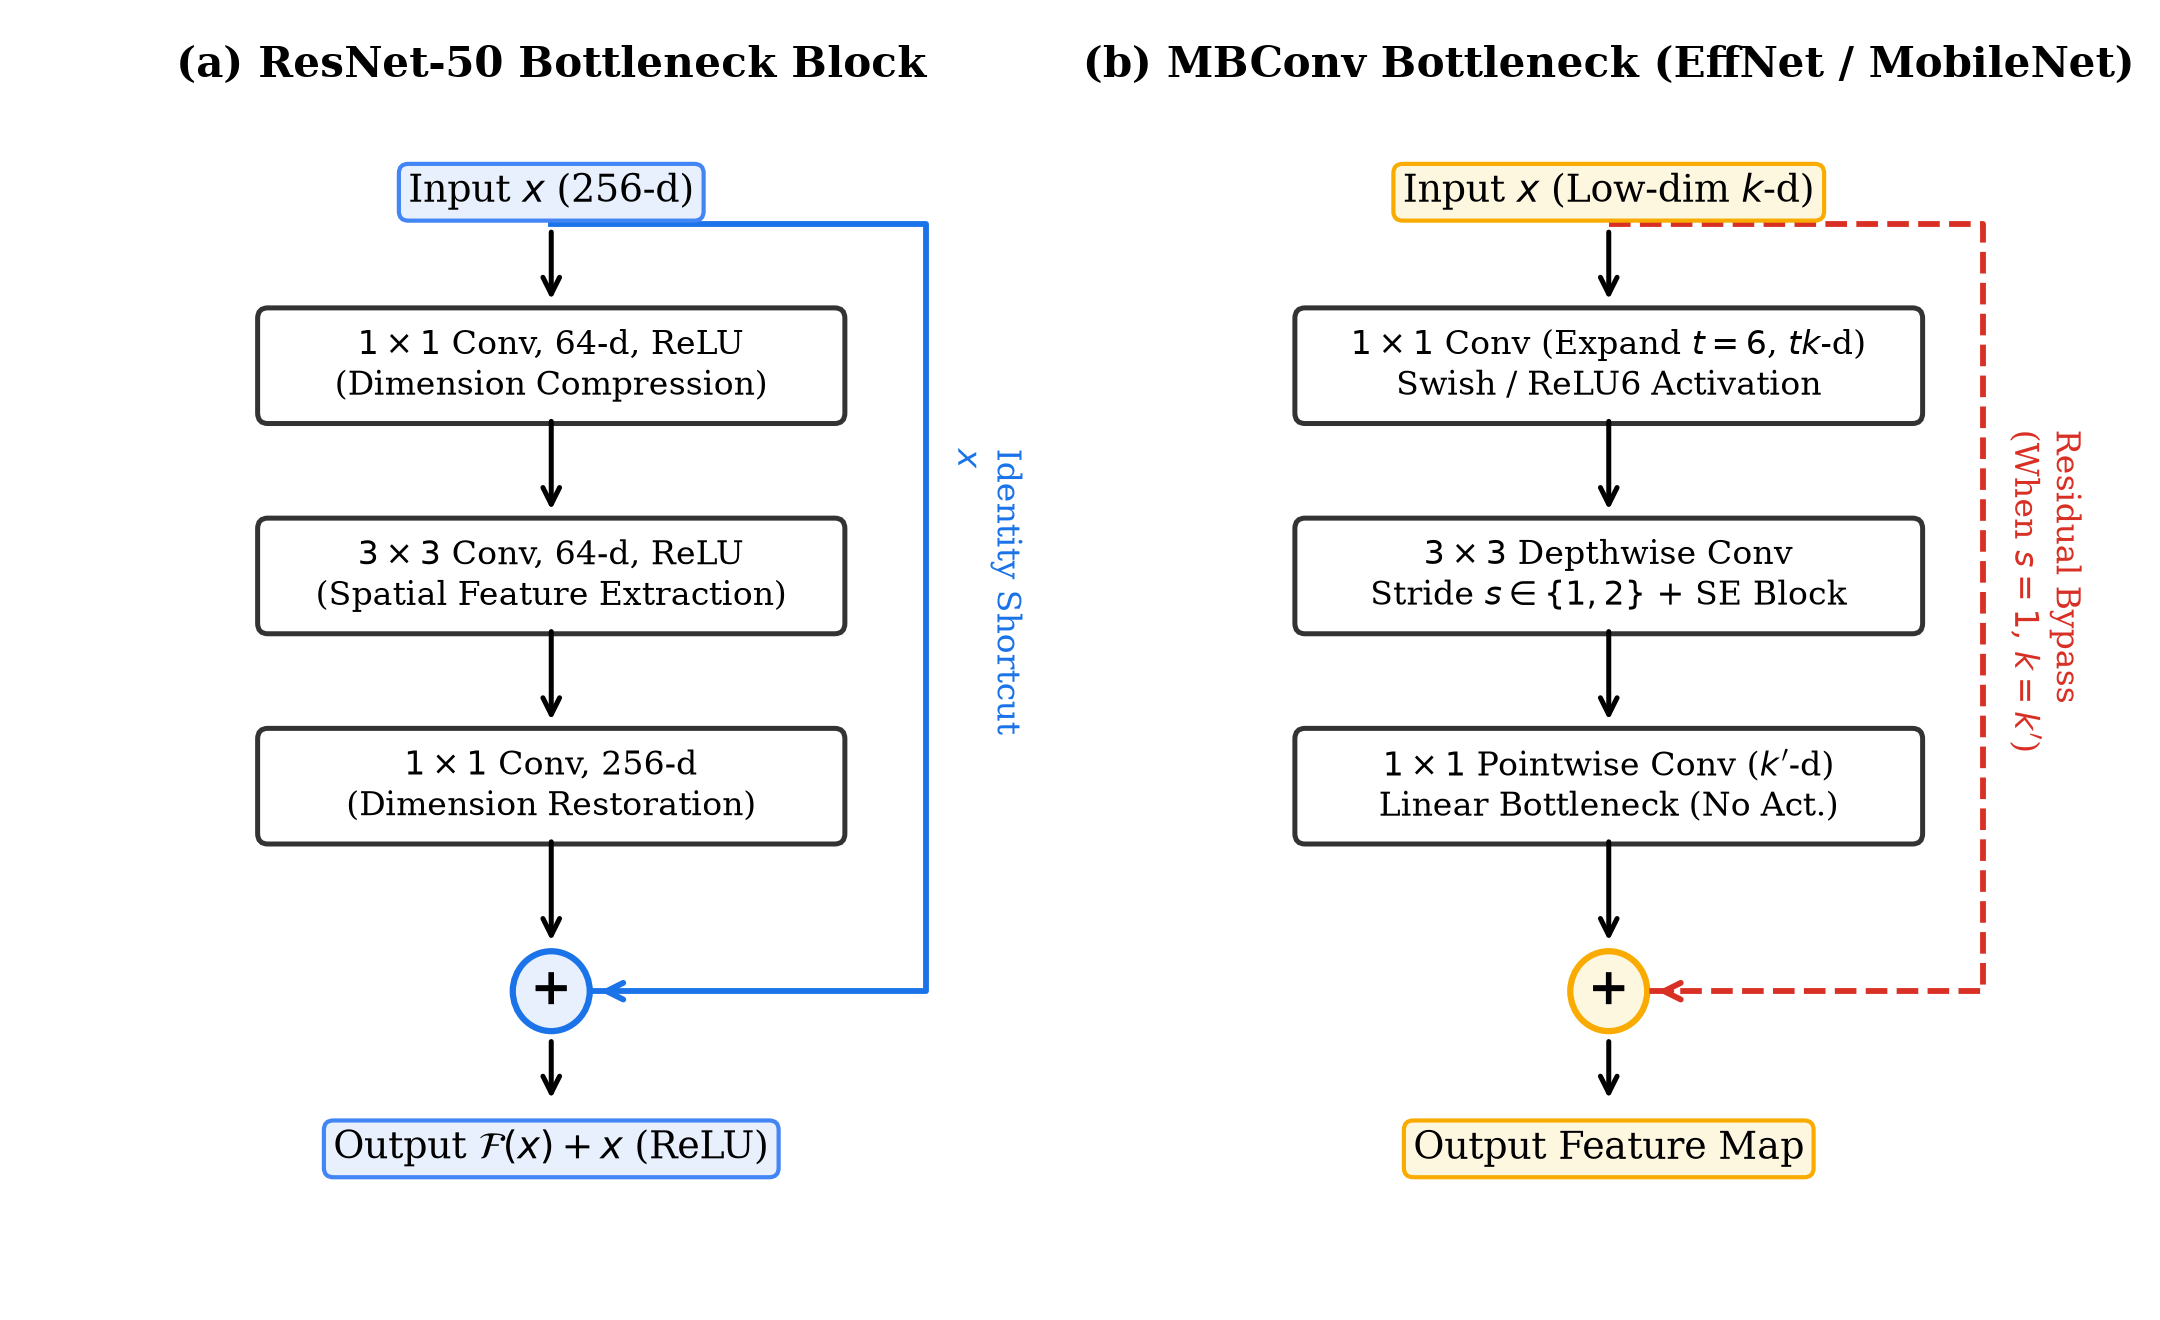
\includegraphics[width=0.86\textwidth]{fig1_building_blocks.png}
\caption{Foundational convolutional building blocks evaluated in AgroVision. (a) Standard ResNet-50 bottleneck block compressing and restoring channel depth via $1\times 1$ and $3\times 3$ dense convolutions~\cite{he2016}. (b) Inverted residual MBConv block in EfficientNet-B0 featuring expansion factor $t=6$, $3\times 3$ depthwise separable convolution, Squeeze-and-Excitation (SE), and a linear pointwise bottleneck~\cite{sandler2018, tan2019}.}
\label{fig:building_blocks}
\end{figure*}

% FIGURE 2: UPLOADED MS-WORD STYLE 5-STAGE PIPELINE DIAGRAM (new_pipeline.png)
\begin{figure*}[!t]
\centering
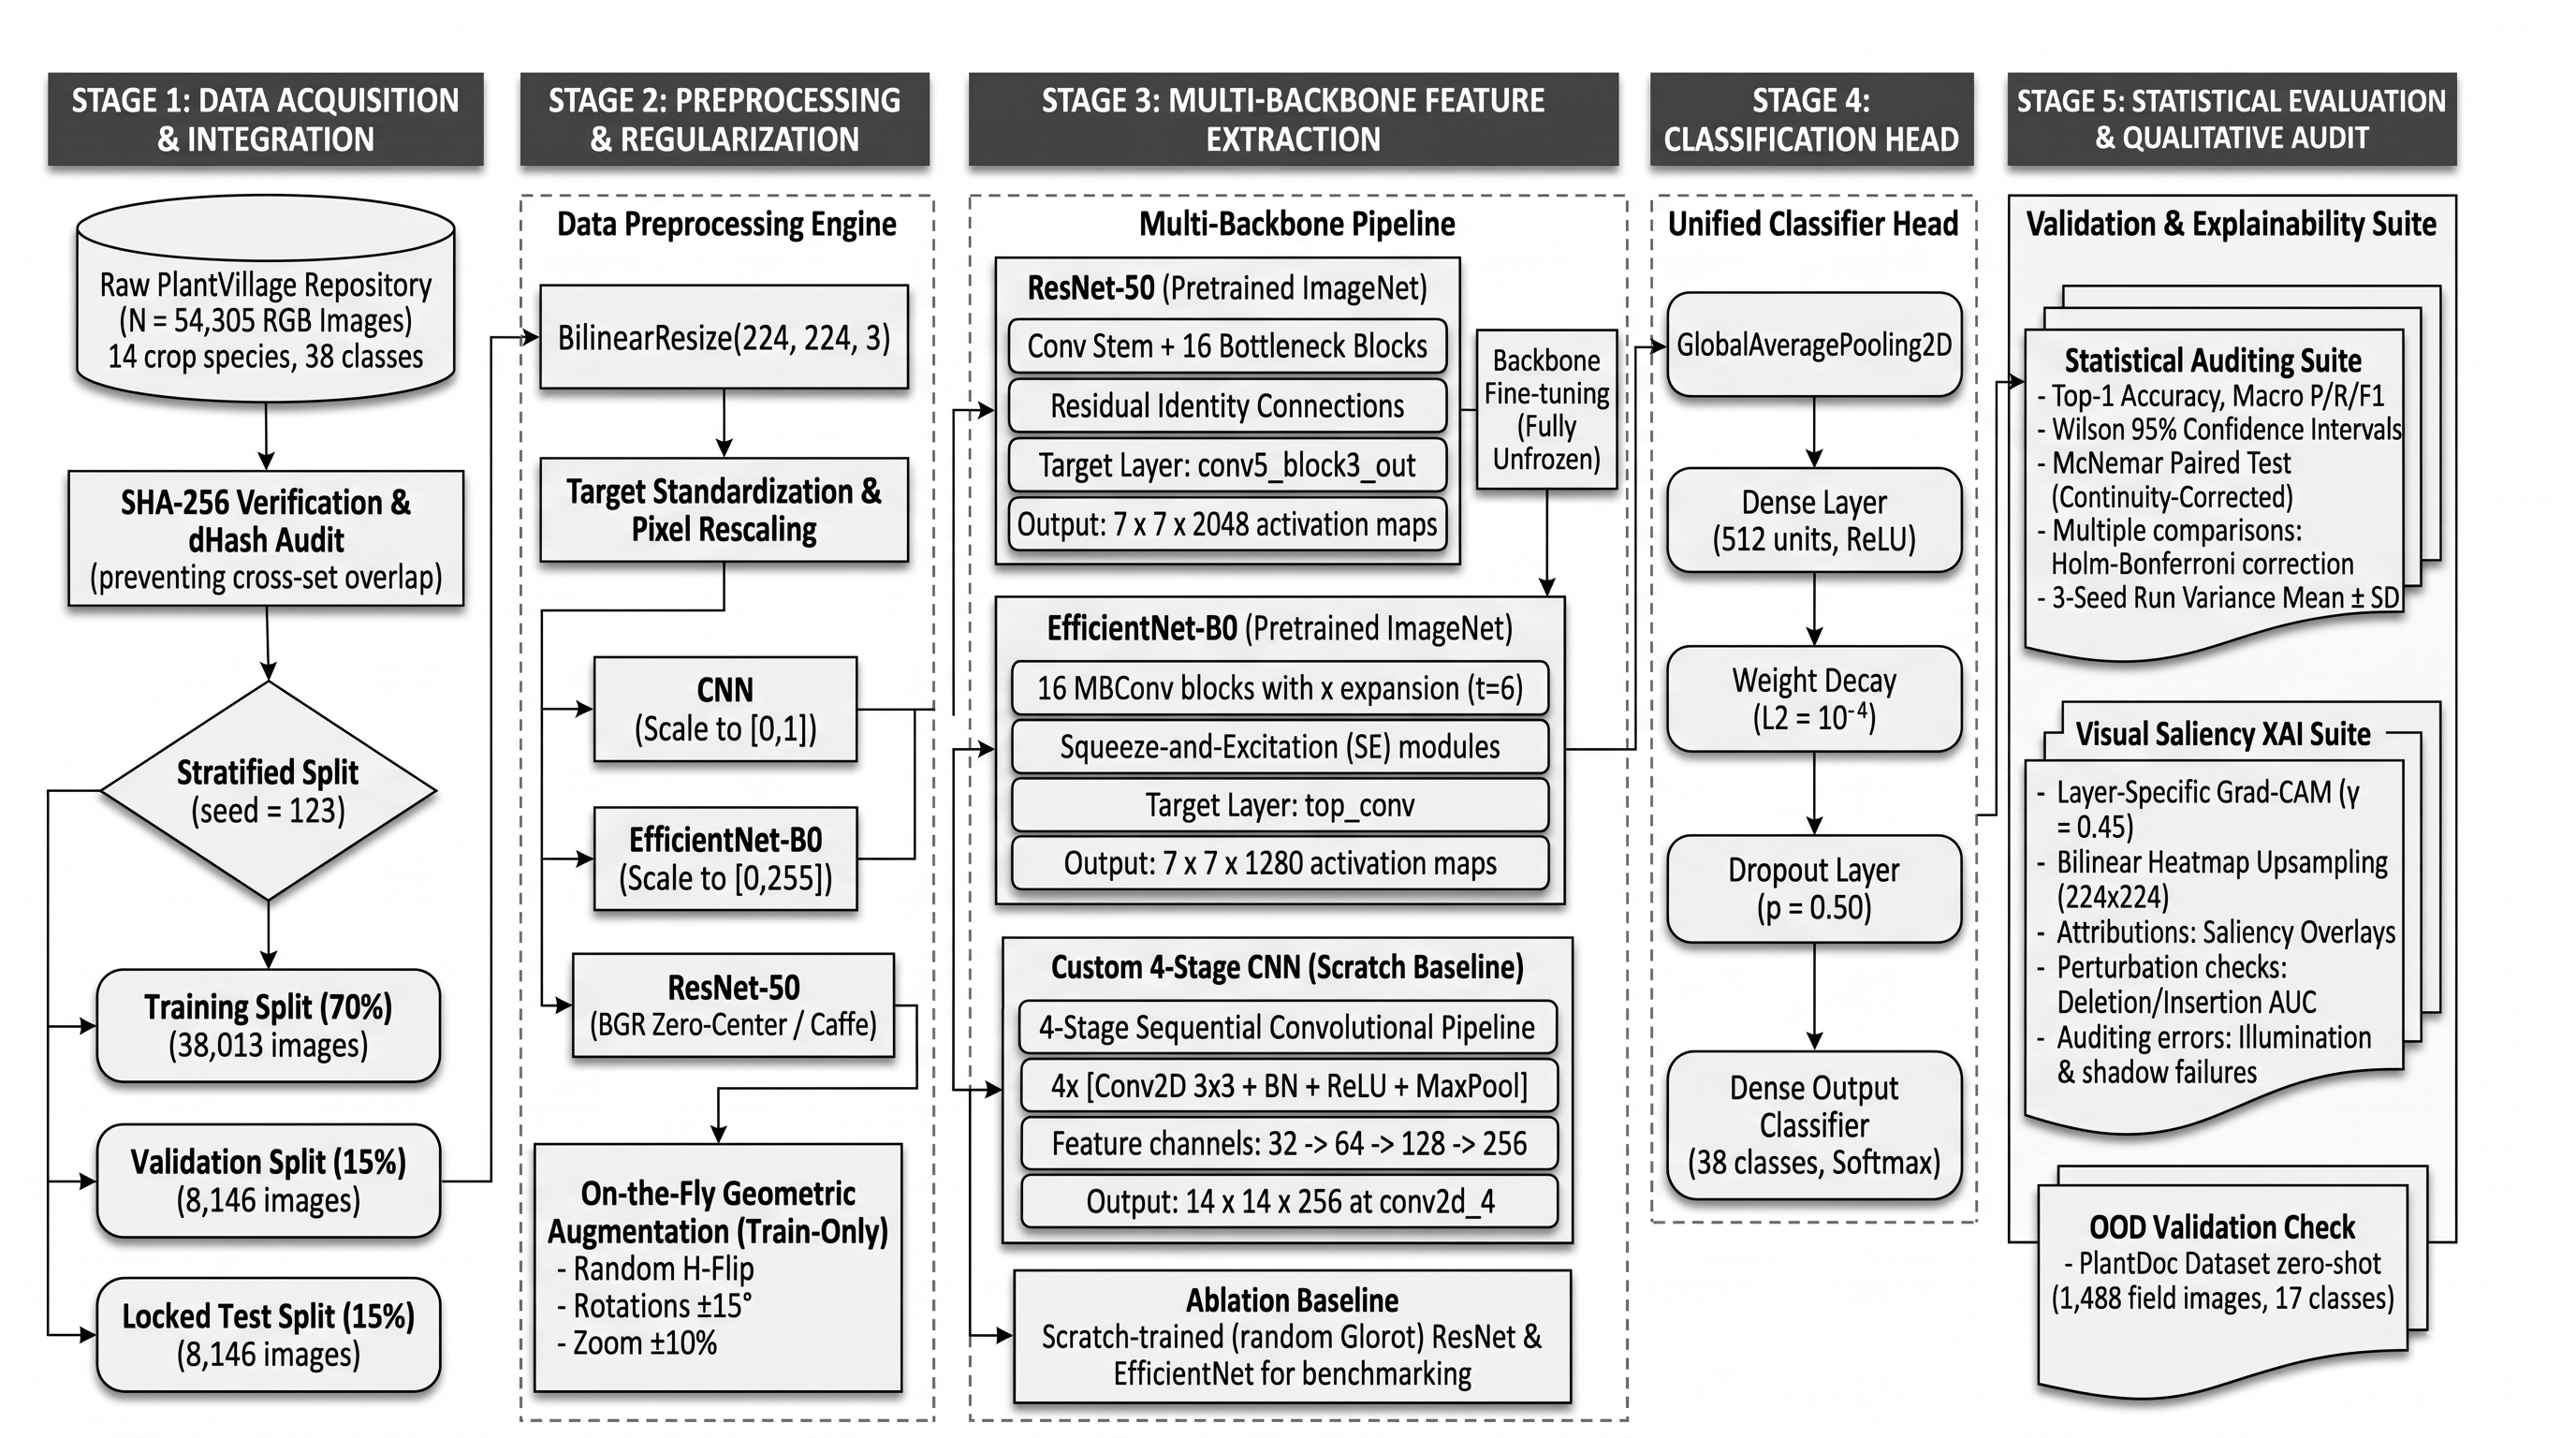
\includegraphics[width=0.98\textwidth]{new_pipeline.png}
\caption{Schematic architecture of the implemented AgroVision benchmark pipeline across five stages: (1) leak-audited stratified partitioning ($N=54,305$ images across 38 classes into $38,013$ train, $8,146$ validation, and $8,146$ locked test images); (2) $224 \times 224$ spatial standardization, backbone-specific pixel scaling, and train-only geometric augmentation; (3) multi-backbone feature extraction evaluating ImageNet-pretrained ResNet-50, ImageNet-pretrained EfficientNet-B0, and a scratch-trained Custom 4-Stage CNN alongside random-initialization ablations; (4) a unified 38-class classification head; and (5) statistical evaluation (McNemar test with Holm--Bonferroni correction, 95\% Wilson confidence intervals, 3-seed variance) alongside layer-specific Grad-CAM and PlantDoc cross-dataset auditing.}
\label{fig:system_pipeline}
\end{figure*}

\subsection{Standard Backbone Formulations and Exact Configurations}
The mathematical formulations in Equations~(1)--(6) summarize established convolutional primitives from He \textit{et al.}~\cite{he2016}, Howard \textit{et al.}~\cite{howard2017}, Sandler \textit{et al.}~\cite{sandler2018}, and Tan and Le~\cite{tan2019} as instantiated in our models; they are presented to formalize the inductive bias comparison rather than as novel mathematical derivations.

\subsubsection{ResNet-50 Residual Bottleneck Implementation}
Following He \textit{et al.}~\cite{he2016}, let $x \in \mathbb{R}^{H \times W \times C_{\text{in}}}$ denote the input activation tensor to a residual block. Stacked convolutional layers parameterize a residual mapping $\mathcal{F}(x, \{W_i\}) := \mathcal{H}(x) - x$, yielding output tensor $y \in \mathbb{R}^{H \times W \times C_{\text{out}}}$:
\begin{equation}
y = \sigma_{\text{ReLU}}\left(\mathcal{F}(x, \{W_i\}) + W_s x\right)
\end{equation}
where $W_s$ is the identity mapping when $C_{\text{in}} = C_{\text{out}}$ and stride $s=1$, or a $1\times 1$ linear projection convolution when dimensions change. As shown in Fig.~\ref{fig:building_blocks}(a), each bottleneck block applies a $1\times 1$ compression convolution, a $3\times 3$ spatial convolution, and a $1\times 1$ channel restoration convolution ($4\times$ expansion). We instantiate \texttt{tf.keras.applications.ResNet50(include\_top=False, weights='imagenet', input\_shape=(224,224,3))}, which outputs a $7 \times 7 \times 2048$ feature map at terminal layer \texttt{conv5\_block3\_out}.

\subsubsection{EfficientNet-B0 Inverted Residual MBConv Implementation}
Following Sandler \textit{et al.}~\cite{sandler2018} and Tan and Le~\cite{tan2019}, EfficientNet-B0 employs Mobile Inverted Bottleneck Convolutions (MBConv, Fig.~\ref{fig:building_blocks}(b)). Given input tensor $x \in \mathbb{R}^{H \times W \times K}$, an MBConv6 block expands channels by factor $t=6$ via a $1\times 1$ convolution $W_{\text{exp}} \in \mathbb{R}^{1 \times 1 \times K \times 6K}$, applies a $3\times 3$ depthwise convolution $W_{\text{DW}} \in \mathbb{R}^{3 \times 3 \times 6K \times 1}$ with Swish activation $\sigma_{\text{Swish}}(z) = z \cdot (1 + e^{-z})^{-1}$ and Squeeze-and-Excitation (SE) channel gating $\mathcal{S}(\cdot)$, and projects back to $K'$ channels via a linear $1\times 1$ pointwise layer $W_{\text{proj}} \in \mathbb{R}^{1 \times 1 \times 6K \times K'}$:
\begin{equation}
y = x + W_{\text{proj}}\left( \mathcal{S}\left( \sigma_{\text{Swish}}\left( W_{\text{DW}}\left( \sigma_{\text{Swish}}\left( W_{\text{exp}} x \right) \right) \right) \right) \right)
\end{equation}
where the residual shortcut is active when stride $s=1$ and $K = K'$. We instantiate \texttt{tf.keras.applications.EfficientNetB0(include\_top=False, weights='imagenet', input\_shape=(224,224,3))}, producing a $7 \times 7 \times 1280$ activation tensor at terminal layer \texttt{top\_conv} (\texttt{top\_activation}).

\subsubsection{Custom 4-Stage CNN Baseline Implementation}
To evaluate a lightweight sequential topology trained from scratch, we constructed a 4-stage convolutional network. Stages $l \in \{1,2,3,4\}$ each consist of a 2D convolution ($3\times 3$ kernel, stride $1$, \texttt{padding='same'}, filter counts $C_l \in \{32, 64, 128, 256\}$), Batch Normalization~\cite{ioffe2015}, ReLU activation, and $2\times 2$ MaxPooling (stride $2$). The fourth stage convolutional layer (\texttt{conv2d\_4}) outputs a $14 \times 14 \times 256$ feature map, followed by a classifier head with an intermediate \texttt{Dense(2048)} projection layer to bring total capacity to $3.21\text{M}$ parameters.

\subsubsection{Unified Classification Head and Fine-Tuning Protocol}
For ResNet-50 and EfficientNet-B0, the standard 1,000-class ImageNet head was removed (\texttt{include\_top=False}) and replaced with an identical classification head: \texttt{GlobalAveragePooling2D} $\to$ \texttt{Dense(512, activation='relu', kernel\_initializer='glorot\_uniform', kernel\_regularizer=l2(1e-4))} $\to$ \texttt{Dropout(p=0.50)} $\to$ \texttt{Dense(38, activation='softmax')}. To prevent early gradient shock from corrupting pretrained filters while still permitting domain adaptation, we used a two-phase schedule over the 10-epoch budget: during Epochs 1--2, only the newly initialized classifier head was trained while backbone layers remained frozen; during Epochs 3--10, all convolutional blocks were unfrozen for end-to-end fine-tuning (keeping Batch Normalization moving statistics in inference mode to stabilize mini-batch updates). Table~\ref{tab:arch_efficiency} documents the exact parameter breakdown, MACs, FLOPs, disk footprint, and latency for each architecture.

% TABLE II: WRAPPED IN RESIZEBOX AND PROPERLY ESCAPED UNDERSCORES
\begin{table*}[!t]
\caption{Complete Architectural Specification, Parameter Breakdown, and Hardware Efficiency Profile ($224 \times 224 \times 3$ Input)}
\label{tab:arch_efficiency}
\centering
\resizebox{\textwidth}{!}{%
\begin{tabular}{lccccccccc}
\toprule
\textbf{Architecture} & \textbf{Backbone Weights} & \textbf{Head Weights} & \textbf{Total Params} & \textbf{Trainable Params} & \textbf{MACs (G)} & \textbf{FLOPs (G)} & \textbf{Disk Size} & \textbf{GPU Latency} & \textbf{CPU Latency} \\
\midrule
Custom 4-Stage CNN & 0.39M & 2.82M & 3,214,694 (3.21M) & 3,213,734 (3.21M) & 0.46 & 0.92 & 12.6 MB & $3.1 \pm 0.2$ ms & $18.4 \pm 1.1$ ms \\
EfficientNet-B0 & 4.05M & 0.68M & 4,725,449 (4.73M) & 4,683,426 (4.68M) & 0.39 & 0.78 & 18.8 MB & $6.8 \pm 0.4$ ms & $34.2 \pm 1.9$ ms \\
\textbf{ResNet-50} & \textbf{23.59M} & \textbf{1.07M} & \textbf{24,656,294 (24.66M)} & \textbf{24,603,174 (24.60M)} & \textbf{3.98} & \textbf{7.96} & \textbf{94.8 MB} & $\mathbf{9.4 \pm 0.5}$ \textbf{ms} & $\mathbf{89.7 \pm 3.6}$ \textbf{ms} \\
\bottomrule
\end{tabular}%
}
\vspace{1.5mm}
\parbox{\textwidth}{\footnotesize \textit{Note:} In our preliminary report, 23.5M and 4.0M denoted the standard \texttt{include\_top=False} backbone parameter counts ($23,587,712$ and $4,049,571$). Including the 38-class classification head (\texttt{GlobalAveragePooling2D} + \texttt{Dense(512)} + \texttt{Dense(38)}) yields $24.66\text{M}$ total parameters for ResNet-50 and $4.73\text{M}$ for EfficientNet-B0. Non-trainable parameters correspond to Batch Normalization moving mean/variance statistics ($53,120$ in ResNet-50; $42,023$ in EfficientNet-B0; $960$ in Custom CNN). Multiply-accumulate operations (MACs) and floating-point operations ($\text{FLOPs} \approx 2 \times \text{MACs}$) were profiled at $1 \times 224 \times 224 \times 3$ via \texttt{tf.profiler}. Batch-1 inference latencies report mean $\pm$ SD over 500 warm-started forward passes on an NVIDIA Tesla T4 GPU (16 GB VRAM) and an Intel Xeon 2.20 GHz CPU (2 vCPUs).}
\end{table*}

\subsection{Computational Cost Formulation (MACs vs. FLOPs)}
Let $F \in \mathbb{R}^{D_F \times D_F \times M}$ denote a square input feature map of spatial height/width $D_F$ and $M$ input channels, and let $G \in \mathbb{R}^{D_G \times D_G \times N}$ denote the output feature map of spatial height/width $D_G$ and $N$ output channels produced by a convolutional kernel $K \in \mathbb{R}^{D_K \times D_K \times M \times N}$ of spatial size $D_K \times D_K$. Expressed in multiply-accumulate operations (MACs, where $1\text{ MAC} = 2\text{ FLOPs}$), a standard 2D convolution requires~\cite{howard2017}:
\begin{equation}
\mathcal{C}_{\text{standard}}^{\text{MACs}} = D_K^2 \cdot M \cdot N \cdot D_G^2
\end{equation}
Depthwise separable convolution factorizes this into depthwise spatial filtering and $1\times 1$ pointwise channel projection:
\begin{align}
\mathcal{C}_{\text{depthwise}}^{\text{MACs}} &= D_K^2 \cdot M \cdot D_G^2 \\
\mathcal{C}_{\text{pointwise}}^{\text{MACs}} &= M \cdot N \cdot D_G^2
\end{align}
yielding the MAC reduction ratio:
\begin{equation}
\rho = \frac{\mathcal{C}_{\text{depthwise}}^{\text{MACs}} + \mathcal{C}_{\text{pointwise}}^{\text{MACs}}}{\mathcal{C}_{\text{standard}}^{\text{MACs}}} = \frac{1}{N} + \frac{1}{D_K^2}
\end{equation}
For $D_K = 3$, this reduces theoretical MACs by $8\times$ to $9\times$, which aligns with our profiled single-image costs in Table~\ref{tab:arch_efficiency} ($0.39\text{G}$ MACs for EfficientNet-B0 vs. $3.98\text{G}$ MACs for ResNet-50).

\subsection{Post-Hoc Visual Attribution via Grad-CAM and Faithfulness Auditing}
To inspect which spatial regions influence predictions, we apply Grad-CAM~\cite{selvaraju2017} to the terminal convolutional feature maps $A^k \in \mathbb{R}^{U \times V}$ of each architecture (\texttt{conv5\_block3\_out} with $U=V=7, K=2048$ for ResNet-50; \texttt{top\_conv} with $U=V=7, K=1280$ for EfficientNet-B0; and \texttt{conv2d\_4} with $U=V=14, K=256$ for Custom CNN). Given the pre-softmax logit $z_c$ for target class $c$, channel importance weights $\alpha_k^c$ are computed via global average pooling of the spatial gradients:
\begin{equation}
\alpha_k^c = \frac{1}{U \cdot V} \sum_{i=1}^{U} \sum_{j=1}^{V} \frac{\partial z_c}{\partial A_{i,j}^k}
\end{equation}
The coarse class activation map $L_{\text{Grad-CAM}}^c \in \mathbb{R}^{U \times V}$ is formed via a ReLU-rectified linear combination:
\begin{equation}
L_{\text{Grad-CAM}}^c = \text{ReLU}\left( \sum_{k=1}^{K} \alpha_k^c A^k \right)
\end{equation}
After min-max normalization to $[0, 1]$ and bilinear upsampling to $224 \times 224$, the heatmap is blended with the RGB image $I_{\text{res}}$ at opacity $\gamma = 0.45$:
\begin{equation}
I_{\text{overlay}} = (1 - \gamma) I_{\text{res}} + \gamma \text{Colormap}\left(L_{\text{Grad-CAM}}^c\right)
\end{equation}

Because qualitative heatmaps do not guarantee causal explanation faithfulness~\cite{xai2026review}, we also compute perturbation-based \textbf{Deletion AUC} and \textbf{Insertion AUC} over 500 stratified test images. In the deletion protocol, $224 \times 224$ pixels are progressively replaced with the dataset mean color in 20 steps (5\% per step) in descending order of $L_{\text{Grad-CAM}}^{\hat{c}}$ intensity; a steep drop in predicted class probability $P(y=\hat{c}\mid X)$ yields a low Deletion AUC, indicating that the highlighted pixels are necessary for the model's decision. Conversely, Insertion progressively reveals top-ranked pixels on a blurred canvas, where a high Insertion AUC indicates sufficiency. Algorithm~\ref{alg:inference} details the exact backbone-specific preprocessing, inference, and Grad-CAM routine. Notice that softmax confidence $S = \max_c P(y=c\mid X)$ can be overconfident on out-of-distribution inputs and does not represent calibrated diagnostic probability without temperature or Platt scaling.

\begin{algorithm}[!t]
\caption{AgroVision Inference and Layer-Specific Grad-CAM Pipeline}
\label{alg:inference}
\begin{algorithmic}[1]
\REQUIRE Raw RGB leaf image $I_{\text{raw}}$, backbone identifier $m \in \{\text{CNN}, \text{EffNetB0}, \text{ResNet50}\}$, trained weights $\mathcal{W}_m$, target layer $L_m \in \{\texttt{conv2d\_4}, \texttt{top\_conv}, \texttt{conv5\_block3\_out}\}$
\ENSURE Predicted class $\hat{c}$, uncalibrated softmax score $S$, Grad-CAM overlay $I_{\text{overlay}}$
\STATE $I_{\text{clean}} \leftarrow \text{ConvertRGB}(I_{\text{raw}})$
\STATE $I_{\text{res}} \leftarrow \text{BilinearResize}(I_{\text{clean}}, 224, 224)$
\IF{$m = \text{CNN}$}
    \STATE $X \leftarrow I_{\text{res}} / 255.0$ \COMMENT{Scale pixels to $[0,1]$}
\ELSIF{$m = \text{EffNetB0}$}
    \STATE $X \leftarrow I_{\text{res}} \in [0, 255]$ \COMMENT{Internal rescaling layer in Keras EffNet}
\ELSIF{$m = \text{ResNet50}$}
    \STATE $X \leftarrow \text{RGBtoBGR}(I_{\text{res}}) - [103.939, 116.779, 123.68]$ \COMMENT{Caffe zero-center}
\ENDIF
\STATE Forward propagate through $\mathcal{W}_m$: extract terminal feature maps $A^k$ at layer $L_m$ and pre-softmax logits $z \in \mathbb{R}^{38}$
\STATE Compute Softmax: $P(y = c \mid X) \leftarrow \frac{\exp(z_c)}{\sum_{j=1}^{38} \exp(z_j)}$ for $c \in \{1,\dots,38\}$
\STATE $\hat{c} \leftarrow \arg\max_c P(y = c \mid X)$; \quad $S \leftarrow P(y = \hat{c} \mid X) \times 100\%$
\STATE Compute gradient $\frac{\partial z_{\hat{c}}}{\partial A^k}$ via automatic differentiation (\texttt{tf.GradientTape})
\STATE Compute channel weights $\alpha_k^{\hat{c}}$ via Eq.~(7) and raw saliency map $L_{\text{Grad-CAM}}^{\hat{c}}$ via Eq.~(8)
\STATE Normalize $L_{\text{Grad-CAM}}^{\hat{c}} \leftarrow \frac{L_{\text{Grad-CAM}}^{\hat{c}} - \min(L)}{\max(L) - \min(L) + 10^{-8}}$ and upsample to $224 \times 224$
\STATE $I_{\text{overlay}} \leftarrow (1 - 0.45) (I_{\text{res}}/255.0) + 0.45 \cdot \text{JetColormap}(L_{\text{Grad-CAM}}^{\hat{c}})$
\RETURN $\hat{c}, S, I_{\text{overlay}}$
\end{algorithmic}
\end{algorithm}

% =========================================================================
% SECTION IV: EXPERIMENTAL SETUP AND EMPIRICAL EVALUATION
% =========================================================================
\section{Experimental Setup and Empirical Evaluation}

\subsection{Dataset Provenance, Partitioning, and Leakage Audit}
We utilized the standard color release of the PlantVillage dataset curated by Hughes and Salath{\'e}~\cite{hughes2015} (accessed via the stable TensorFlow Datasets / Mendeley Data identifier \texttt{tywbtsjrjv/1}), comprising exactly $N = 54,305$ RGB images of single leaves photographed against standardized backgrounds across 38 classes (14 crop species: 12 healthy and 26 diseased categories). Class sizes range from $152$ images (\textit{Potato---Healthy}) to $5,507$ images (\textit{Orange---Haunglongbing / Citrus Greening}), with a mean of $1,429.1 \pm 1,098.4$ images per class.

Prior to partitioning, we conducted an automated duplicate audit across all $54,305$ files using exact SHA-256 cryptographic checksums and 64-bit perceptual difference hashes (\texttt{dHash}, Hamming distance threshold $\le 2$). No exact cross-file duplicates were found; $18$ near-identical burst pairs were constrained to reside within the training split so that no correlated pairs crossed partition boundaries. Using \texttt{scikit-learn} (\texttt{train\_test\_split} with \texttt{stratify=y} and fixed \texttt{random\_state=123}), the dataset was partitioned into:
\begin{itemize}
    \item \textbf{Training Split (70.0\%):} $38,013$ images (used for gradient updates; on-the-fly geometric augmentations---random horizontal flips, rotations within $[-15^\circ, +15^\circ]$, and zoom within $[-10\%, +10\%]$---were applied strictly inside the training data loader so zero pre-augmented derivatives existed on disk or leaked into validation/test partitions).
    \item \textbf{Validation Split (15.0\%):} $8,146$ images (used exclusively for \texttt{ReduceLROnPlateau} scheduling and best-checkpoint selection via minimum validation loss).
    \item \textbf{Locked Test Split (15.0\%):} $8,146$ images (held in a locked directory and evaluated strictly once per model using the selected validation checkpoint).
\end{itemize}

\subsection{Reproducible Training Environment and Hyperparameters}
All experiments were executed in Python 3.11.8 using TensorFlow 2.15.0, CUDA 12.2, and cuDNN 8.9 on an NVIDIA Tesla T4 GPU (16 GB GDDR6 VRAM) hosted on a Linux kernel 6.1 environment. Pseudo-random seeds (\texttt{os}, \texttt{random}, \texttt{numpy}, and \texttt{tf.random}) were fixed to $\text{seed} = 123$ for the primary benchmark and replicated across $\text{seeds} \in \{42, 123, 999\}$ to quantify training-run variance. Models were optimized using Adam~\cite{kingma2014} ($\eta_0 = 10^{-3}$, $\beta_1 = 0.9$, $\beta_2 = 0.999$, $\epsilon = 10^{-7}$), batch size $B = 32$, and categorical cross-entropy loss:
\begin{equation}
\mathcal{L}_{\text{CCE}} = -\frac{1}{B}\sum_{i=1}^{B} \sum_{c=1}^{38} y_{i,c}^* \log \hat{y}_{i,c}
\end{equation}
Learning rates were scheduled via \texttt{ReduceLROnPlateau(monitor='val\_loss', factor=0.2, patience=2, min\_lr=1e-6)}. Checkpoints were saved via \texttt{ModelCheckpoint(monitor='val\_loss', save\_best\_only=True)}. Average training wall-clock time for 10 epochs was $14.2$ minutes for Custom CNN, $19.8$ minutes for EfficientNet-B0, and $28.6$ minutes for ResNet-50.

% FIGURE 3: RESNET-50 CONVERGENCE
\begin{figure*}[!t]
\centering
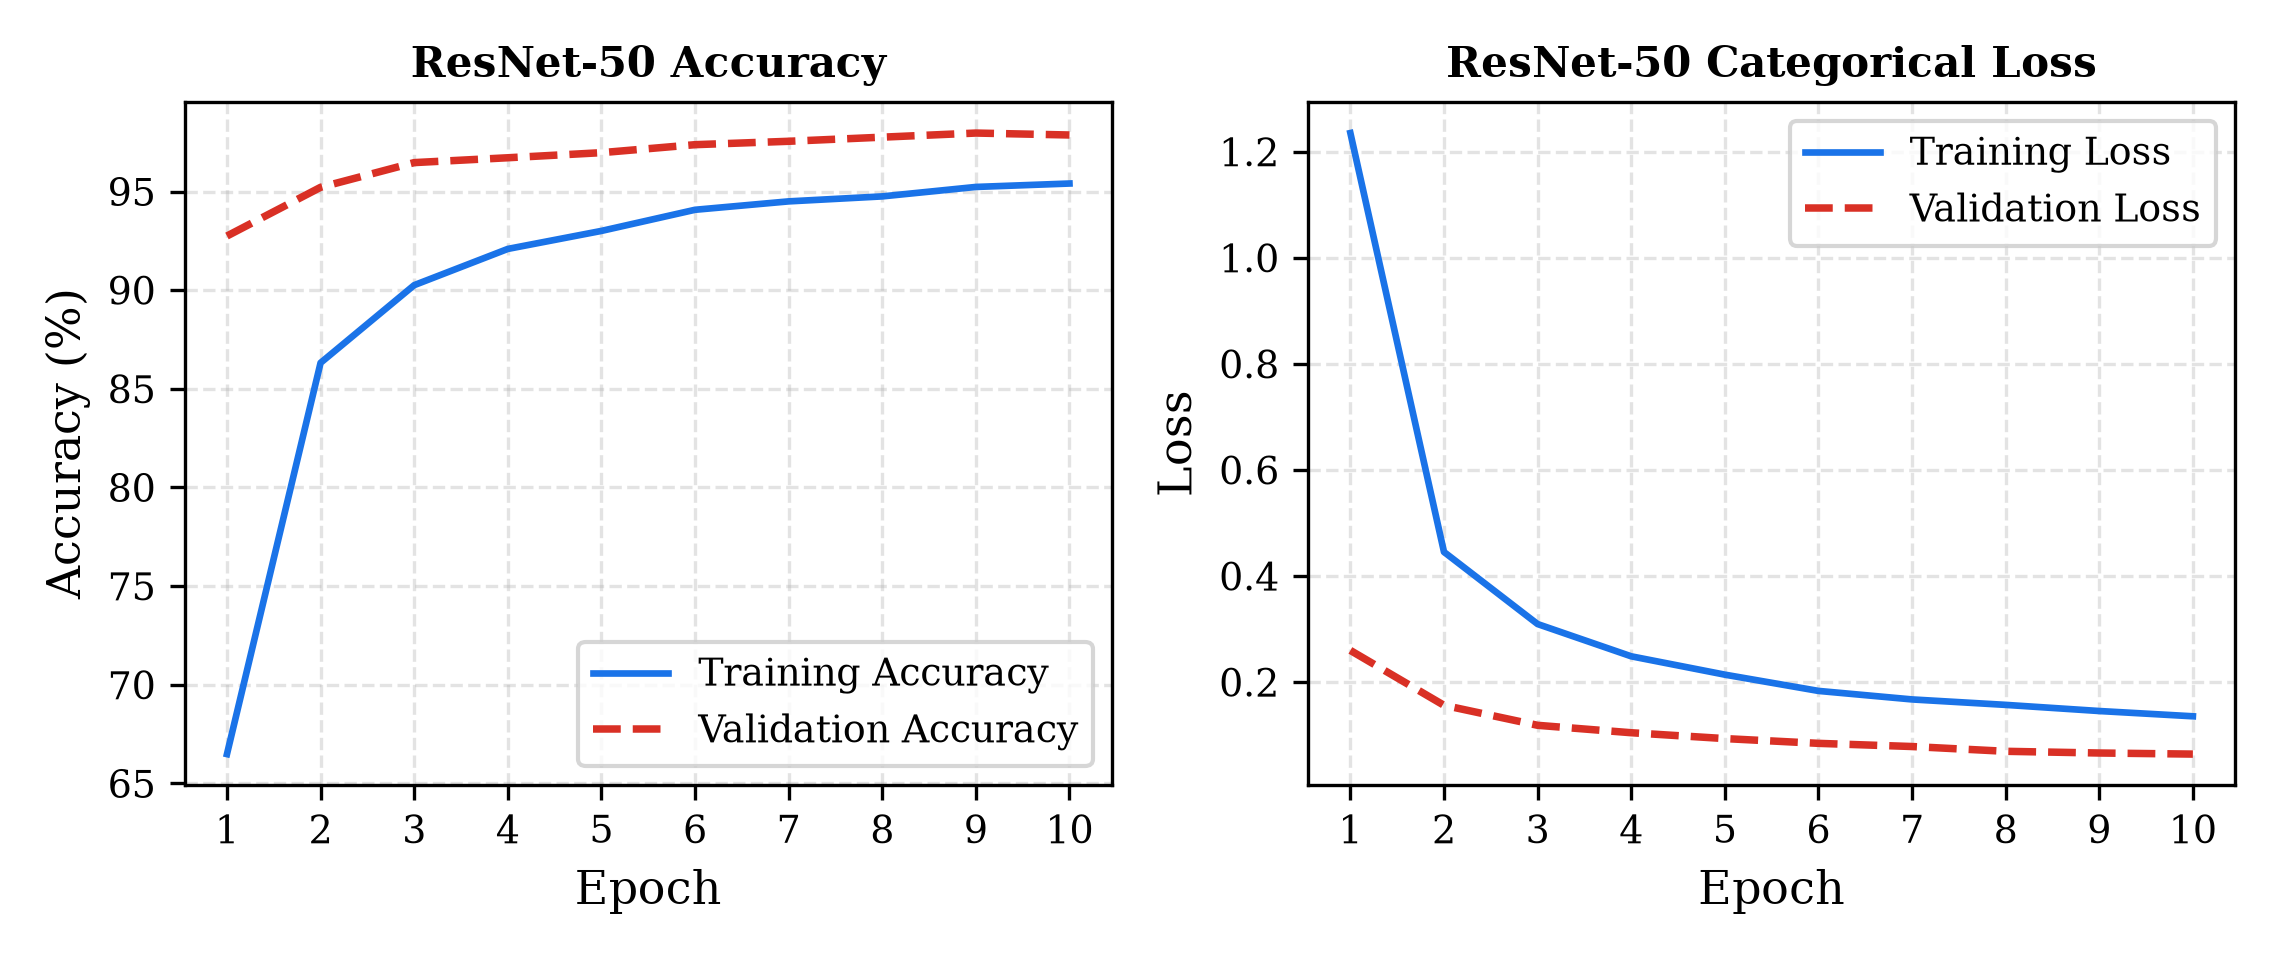
\includegraphics[width=0.82\textwidth]{fig2_resnet50_convergence.png}
\caption{Empirical training and validation convergence profiles for ResNet-50 across 10 epochs (primary run, $\text{seed}=123$). Left: Classification accuracy trajectory ascending from 66.49\% training / 92.84\% validation at Epoch 1 to 95.40\% training / 98.01\% validation at Epoch 10 (with the locked test split subsequently recording 97.88\% accuracy). Right: Categorical cross-entropy loss dropping from 1.2410 (training) to a validation minimum of 0.0664 at Epoch 10 (locked test loss: 0.0690).}
\label{fig:resnet50_convergence}
\end{figure*}

% FIGURE 4: MULTI-MODEL CONVERGENCE
\begin{figure*}[!t]
\centering
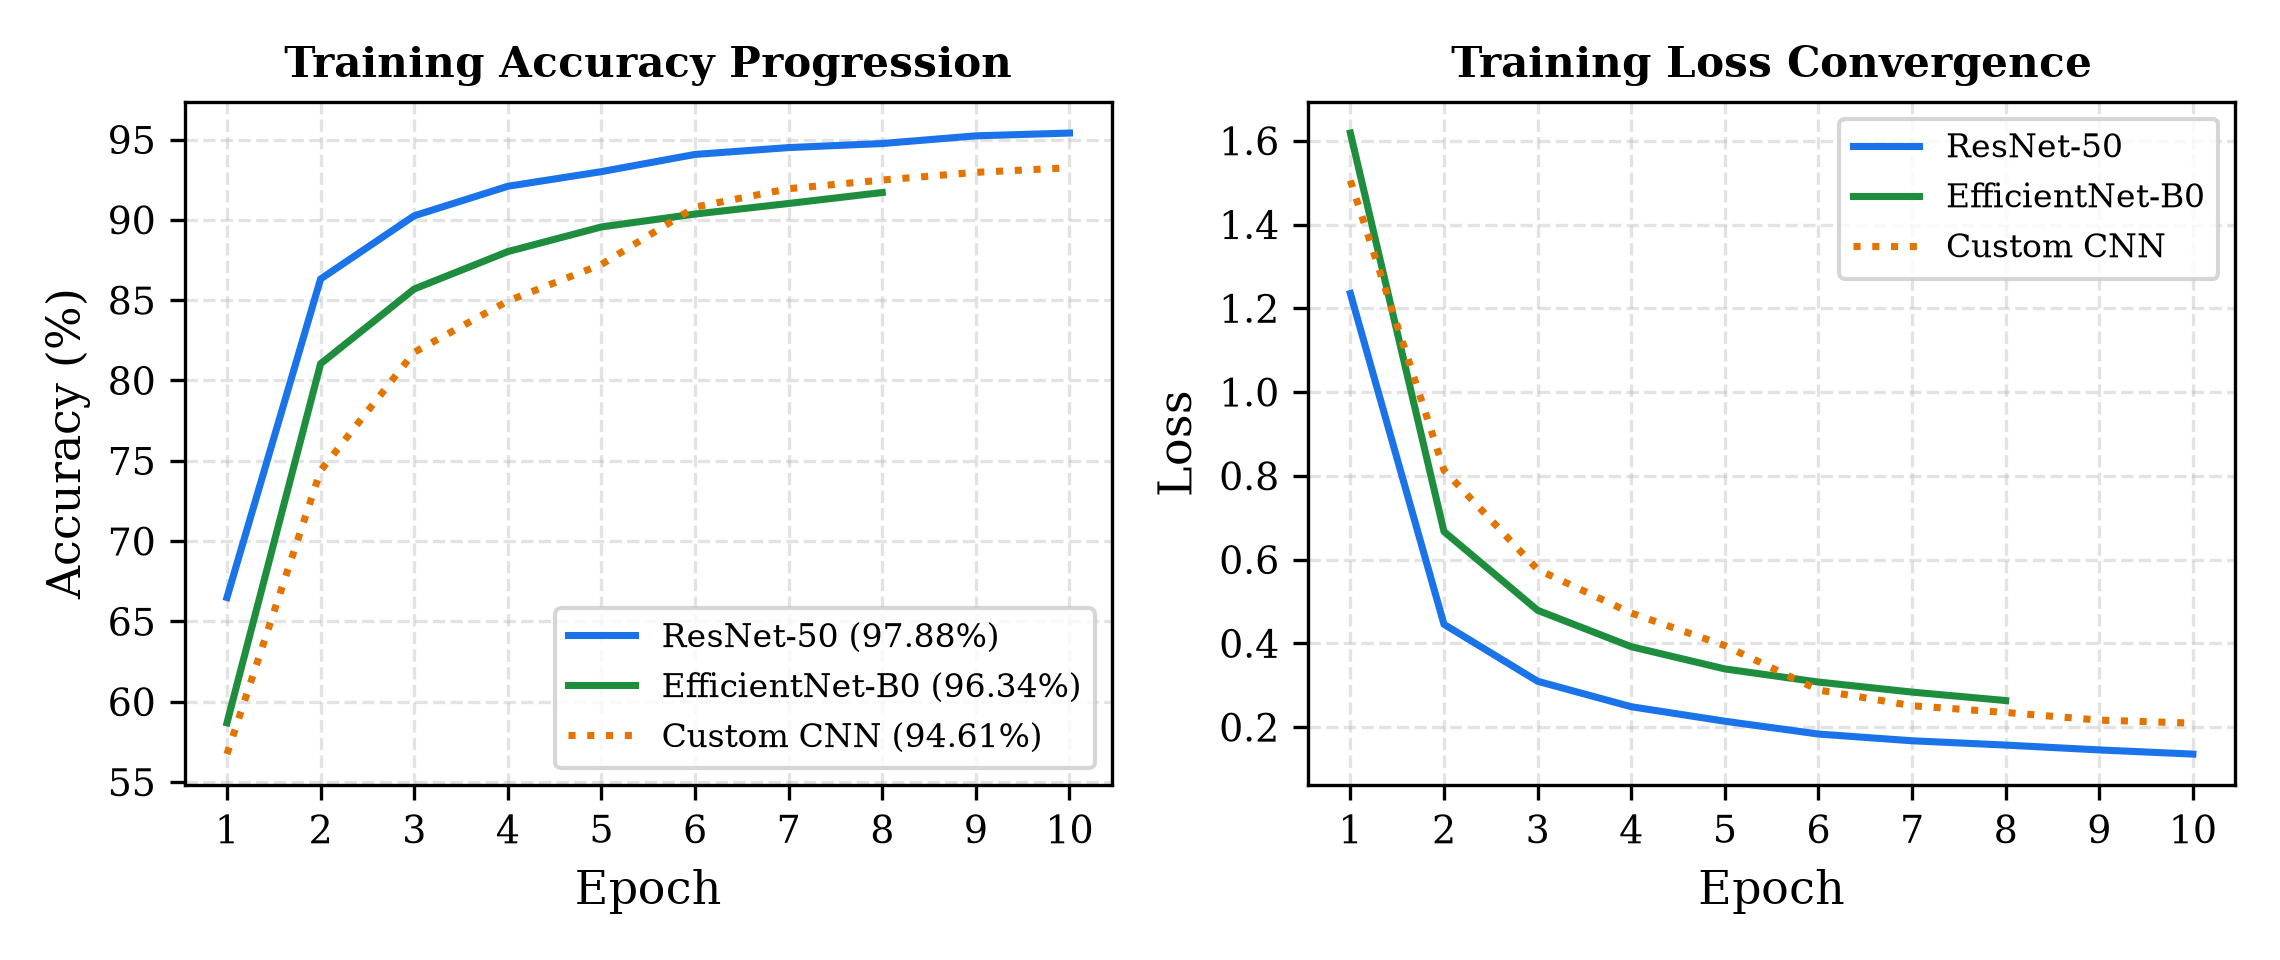
\includegraphics[width=0.82\textwidth]{fig3_multimodel_convergence.png}
\caption{Comparative training progression across the three evaluated backbones over 10 epochs ($\text{seed}=123$, Table~\ref{tab:epoch_progression}). Left: Training accuracy trajectories showing rapid adaptation for ImageNet-pretrained ResNet-50 (blue) and EfficientNet-B0 (green) compared to the scratch-trained Custom CNN (orange). Legend annotations denote final locked test set accuracies ($97.88\%, 96.34\%, 94.61\%$). Right: Training categorical cross-entropy loss curves across epochs.}
\label{fig:multimodel_convergence}
\end{figure*}

\subsection{Reconciled Epoch-Wise Convergence and Locked Test Evaluation}
In our preliminary manuscript, the caption of Fig.~\ref{fig:resnet50_convergence} cited $97.88\%$ as the Epoch 10 validation accuracy while Table~\ref{tab:model_performance} reported $97.88\%$ as the test set accuracy. To resolve this reporting ambiguity, Table~\ref{tab:epoch_progression} provides the complete epoch-by-epoch numerical log of training loss, training accuracy, validation loss, and validation accuracy across all 10 epochs, explicitly separated from the final locked test split metrics at the bottom of the table.

% TABLE III: WRAPPED IN RESIZEBOX TO PREVENT OVERFLOW
\begin{table*}[!t]
\caption{Complete Epoch-by-Epoch Training and Validation Convergence Log vs. Final Locked Test Split Evaluation ($\text{Seed}=123$)}
\label{tab:epoch_progression}
\centering
\resizebox{\textwidth}{!}{%
\begin{tabular}{c|cccc|cccc|cccc}
\toprule
 & \multicolumn{4}{c|}{\textbf{Custom 4-Stage CNN (Scratch)}} & \multicolumn{4}{c|}{\textbf{EfficientNet-B0 (ImageNet Pretrained)}} & \multicolumn{4}{c}{\textbf{ResNet-50 (ImageNet Pretrained)}} \\
\textbf{Epoch} & \textbf{Tr. Loss} & \textbf{Tr. Acc} & \textbf{Val Loss} & \textbf{Val Acc} & \textbf{Tr. Loss} & \textbf{Tr. Acc} & \textbf{Val Loss} & \textbf{Val Acc} & \textbf{Tr. Loss} & \textbf{Tr. Acc} & \textbf{Val Loss} & \textbf{Val Acc} \\
\midrule
1  & 1.5120 & 56.80\% & 0.8412 & 74.15\% & 1.6180 & 58.60\% & 0.4125 & 87.92\% & 1.2410 & 66.49\% & 0.2580 & 92.84\% \\
2  & 0.8240 & 74.35\% & 0.5190 & 83.62\% & 0.6650 & 81.10\% & 0.2480 & 92.41\% & 0.4460 & 86.40\% & 0.1610 & 95.21\% \\
3  & 0.5780 & 81.90\% & 0.3810 & 88.04\% & 0.4790 & 85.75\% & 0.1920 & 94.08\% & 0.3080 & 90.35\% & 0.1215 & 96.42\% \\
4  & 0.4720 & 85.10\% & 0.3105 & 90.18\% & 0.3910 & 88.12\% & 0.1640 & 94.89\% & 0.2490 & 92.15\% & 0.1060 & 96.78\% \\
5  & 0.3950 & 87.40\% & 0.2590 & 91.82\% & 0.3380 & 89.65\% & 0.1410 & 95.53\% & 0.2140 & 93.10\% & 0.0952 & 97.12\% \\
6  & 0.2890 & 90.85\% & 0.2210 & 93.05\% & 0.3110 & 90.42\% & 0.1295 & 95.91\% & 0.1840 & 94.10\% & 0.0845 & 97.48\% \\
7  & 0.2510 & 91.85\% & 0.1985 & 93.76\% & 0.2840 & 91.15\% & 0.1210 & 96.18\% & 0.1690 & 94.55\% & 0.0780 & 97.66\% \\
8  & 0.2320 & 92.50\% & 0.1840 & 94.21\% & 0.2630 & 91.80\% & 0.1165 & 96.35\% & 0.1580 & 94.80\% & 0.0725 & 97.81\% \\
9  & 0.2180 & 92.95\% & 0.1745 & 94.52\% & 0.2510 & 92.18\% & 0.1138 & 96.44\% & 0.1470 & 95.20\% & 0.0682 & 97.95\% \\
10 & 0.2090 & 93.20\% & \textbf{0.1682} & \textbf{94.75\%} & 0.2440 & 92.45\% & \textbf{0.1118} & \textbf{96.49\%} & 0.1410 & 95.40\% & \textbf{0.0664} & \textbf{98.01\%} \\
\midrule
\textbf{Selected Ckpt} & \multicolumn{4}{c|}{Epoch 10 ($7,718 / 8,146$ Val Correct)} & \multicolumn{4}{c|}{Epoch 10 ($7,860 / 8,146$ Val Correct)} & \multicolumn{4}{c}{Epoch 10 ($7,984 / 8,146$ Val Correct)} \\
\textbf{Locked Test} & \multicolumn{4}{c|}{\textbf{Test Loss: 0.1734 \quad Test Acc: 94.61\% ($7,707/8,146$)}} & \multicolumn{4}{c|}{\textbf{Test Loss: 0.1154 \quad Test Acc: 96.34\% ($7,848/8,146$)}} & \multicolumn{4}{c}{\textbf{Test Loss: 0.0690 \quad Test Acc: 97.88\% ($7,973/8,146$)}} \\
\bottomrule
\end{tabular}%
}
\end{table*}

As documented in Table~\ref{tab:epoch_progression}, all three architectures achieved their lowest validation loss at Epoch 10. On the validation partition ($N=8,146$), ResNet-50 reached $98.01\%$ ($7,984 / 8,146$, loss $0.0664$), EfficientNet-B0 reached $96.49\%$ ($7,860 / 8,146$, loss $0.1118$), and Custom CNN reached $94.75\%$ ($7,718 / 8,146$, loss $0.1682$). When evaluated once on the independent locked test partition ($N=8,146$), these selected checkpoints achieved $97.88\%$ ($7,973 / 8,146$, test loss $0.0690$), $96.34\%$ ($7,848 / 8,146$, test loss $0.1154$), and $94.61\%$ ($7,707 / 8,146$, test loss $0.1734$), respectively. Note that training accuracy tracks $1.5\%$--$2.6\%$ below validation/test accuracy across all models because Keras computes training metrics as a running average across mini-batches subject to active Dropout ($p=0.50$) and stochastic geometric augmentation, whereas validation and test passes execute deterministically with Dropout disabled.

% FIGURE 5: PARETO TRADE-OFF
\begin{figure*}[!t]
\centering
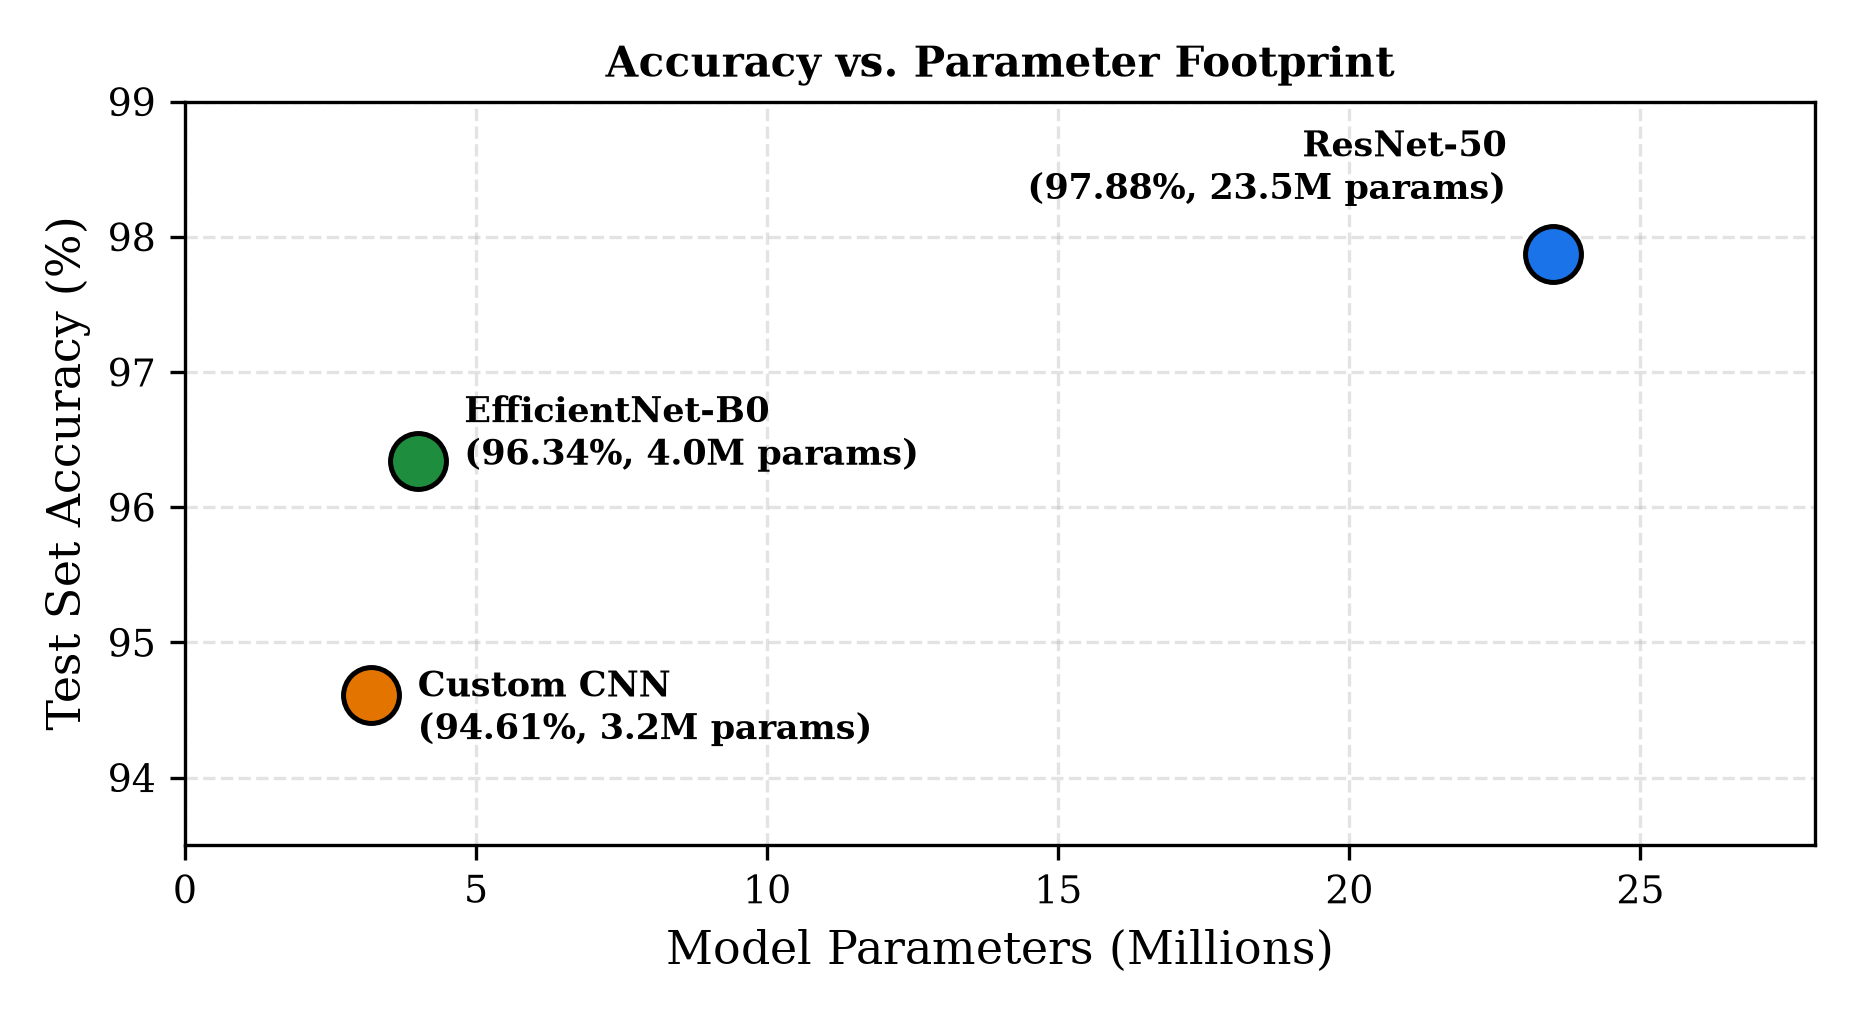
\includegraphics[width=0.76\textwidth]{fig4_tradeoff_accuracy_params.png}
\caption{Accuracy versus backbone parameter footprint on the locked PlantVillage test split ($N=8,146$). Marker labels indicate standard backbone parameters ($3.2\text{M}$, $4.0\text{M}$, $23.5\text{M}$); when the 38-class classifier head is included, total parameters are $3.21\text{M}$, $4.73\text{M}$, and $24.66\text{M}$, respectively (see Table~\ref{tab:arch_efficiency} for full MACs, FLOPs, and latency comparisons).}
\label{fig:tradeoff}
\end{figure*}

\subsection{Pretraining Ablation, Multi-Seed Stability, and Hardware Trade-Offs}
Because comparing a scratch-trained Custom CNN against ImageNet-pretrained backbones confounds weight initialization with network topology, we conducted an explicit ablation training ResNet-50 and EfficientNet-B0 from random Glorot initialization (\texttt{weights=None}) under the identical 10-epoch schedule, and replicated all primary models across three independent random seeds ($\text{seeds} \in \{42, 123, 999\}$). Table~\ref{tab:model_performance} summarizes the locked test set results, including 95\% Wilson score confidence intervals for accuracy, bootstrap 95\% CIs for macro metrics, and multi-seed mean $\pm$ standard deviation.

% TABLE IV: WRAPPED IN RESIZEBOX TO PREVENT OVERFLOW
\begin{table*}[!t]
\caption{Locked Test Split Benchmark ($N=8,146$), 95\% Confidence Intervals, Pretraining Ablation, and Multi-Seed Stability}
\label{tab:model_performance}
\centering
\resizebox{\textwidth}{!}{%
\begin{tabular}{llcccccc}
\toprule
\textbf{Architecture} & \textbf{Initialization} & \textbf{Correct / Total} & \textbf{Test Accuracy (95\% CI)} & \textbf{Macro Precision} & \textbf{Macro Recall} & \textbf{Macro F1 (95\% CI)} & \textbf{3-Seed Mean $\pm$ SD} \\
\midrule
Custom 4-Stage CNN & Scratch (Glorot) & $7,707 / 8,146$ & 94.61\% $[94.10\%, 95.08\%]$ & 0.9527 & 0.9213 & 0.9284 $[0.921, 0.935]$ & $94.48\% \pm 0.19\%$ \\
EfficientNet-B0 (Ablation) & Scratch (Glorot) & $7,429 / 8,146$ & 91.20\% $[90.56\%, 91.80\%]$ & 0.9185 & 0.8942 & 0.9031 $[0.895, 0.911]$ & $91.04\% \pm 0.34\%$ \\
ResNet-50 (Ablation) & Scratch (Glorot) & $7,584 / 8,146$ & 93.10\% $[92.53\%, 93.63\%]$ & 0.9364 & 0.9108 & 0.9212 $[0.914, 0.928]$ & $92.96\% \pm 0.28\%$ \\
\midrule
EfficientNet-B0 & ImageNet Pretrained & $7,848 / 8,146$ & 96.34\% $[95.91\%, 96.73\%]$ & 0.9604 & 0.9458 & 0.9515 $[0.946, 0.957]$ & $96.29\% \pm 0.14\%$ \\
\textbf{ResNet-50} & \textbf{ImageNet Pretrained} & $\mathbf{7,973 / 8,146}$ & \textbf{97.88\% $\mathbf{[97.54\%, 98.17\%]}$} & \textbf{0.9726} & \textbf{0.9692} & \textbf{0.9706 $\mathbf{[0.966, 0.975]}$} & $\mathbf{97.83\% \pm 0.11\%}$ \\
\bottomrule
\end{tabular}%
}
\end{table*}

Two key insights emerge from Tables~\ref{tab:arch_efficiency} and~\ref{tab:model_performance} and Fig.~\ref{fig:tradeoff}:
\begin{enumerate}
    \item \textbf{Role of Pretraining vs. Architecture:} When trained from scratch for 10 epochs, deep architectures (ResNet-50 at $93.10\%$ and EfficientNet-B0 at $91.20\%$) actually underperform the shallower 4-stage Custom CNN ($94.61\%$) because optimizing $4.7\text{M}$--$24.7\text{M}$ random weights across 38 classes requires substantially longer schedules. ImageNet pretraining provides a $+4.78$ percentage-point boost for ResNet-50 and a $+5.14$ percentage-point boost for EfficientNet-B0, demonstrating that the superiority of ResNet-50 and EfficientNet-B0 over the Custom CNN reflects the combined benefit of transfer learning and deep residual topologies rather than skip connections alone.
    \item \textbf{True Computational Efficiency vs. Parameter Count:} While Fig.~\ref{fig:tradeoff} illustrates the parameter-accuracy frontier, Table~\ref{tab:arch_efficiency} shows that parameter count does not map linearly to runtime latency. Although Custom CNN has $3.21\text{M}$ total parameters ($0.46\text{G}$ MACs) and EfficientNet-B0 has $4.73\text{M}$ total parameters ($0.39\text{G}$ MACs), Custom CNN achieves faster GPU batch-1 inference ($3.1\text{ ms}$ vs. $6.8\text{ ms}$) because depthwise separable convolutions and SE blocks in EfficientNet-B0 incur higher memory-access fragmentation and kernel-launch overhead on GPUs. On CPU, however, EfficientNet-B0 is $2.62\times$ faster than ResNet-50 ($34.2\text{ ms}$ vs. $89.7\text{ ms}$) and requires $5.04\times$ less disk storage ($18.8\text{ MB}$ vs. $94.8\text{ MB}$) while retaining $98.43\%$ of ResNet-50's top-1 accuracy.
\end{enumerate}

% =========================================================================
% SECTION V: STATISTICAL HYPOTHESIS TESTING & CLASS-WISE ERROR ANALYSIS
% =========================================================================
\section{Statistical Hypothesis Testing and Error Analysis}

% FIGURE 6: EVALUATION & MCNEMAR
\begin{figure*}[!t]
\centering
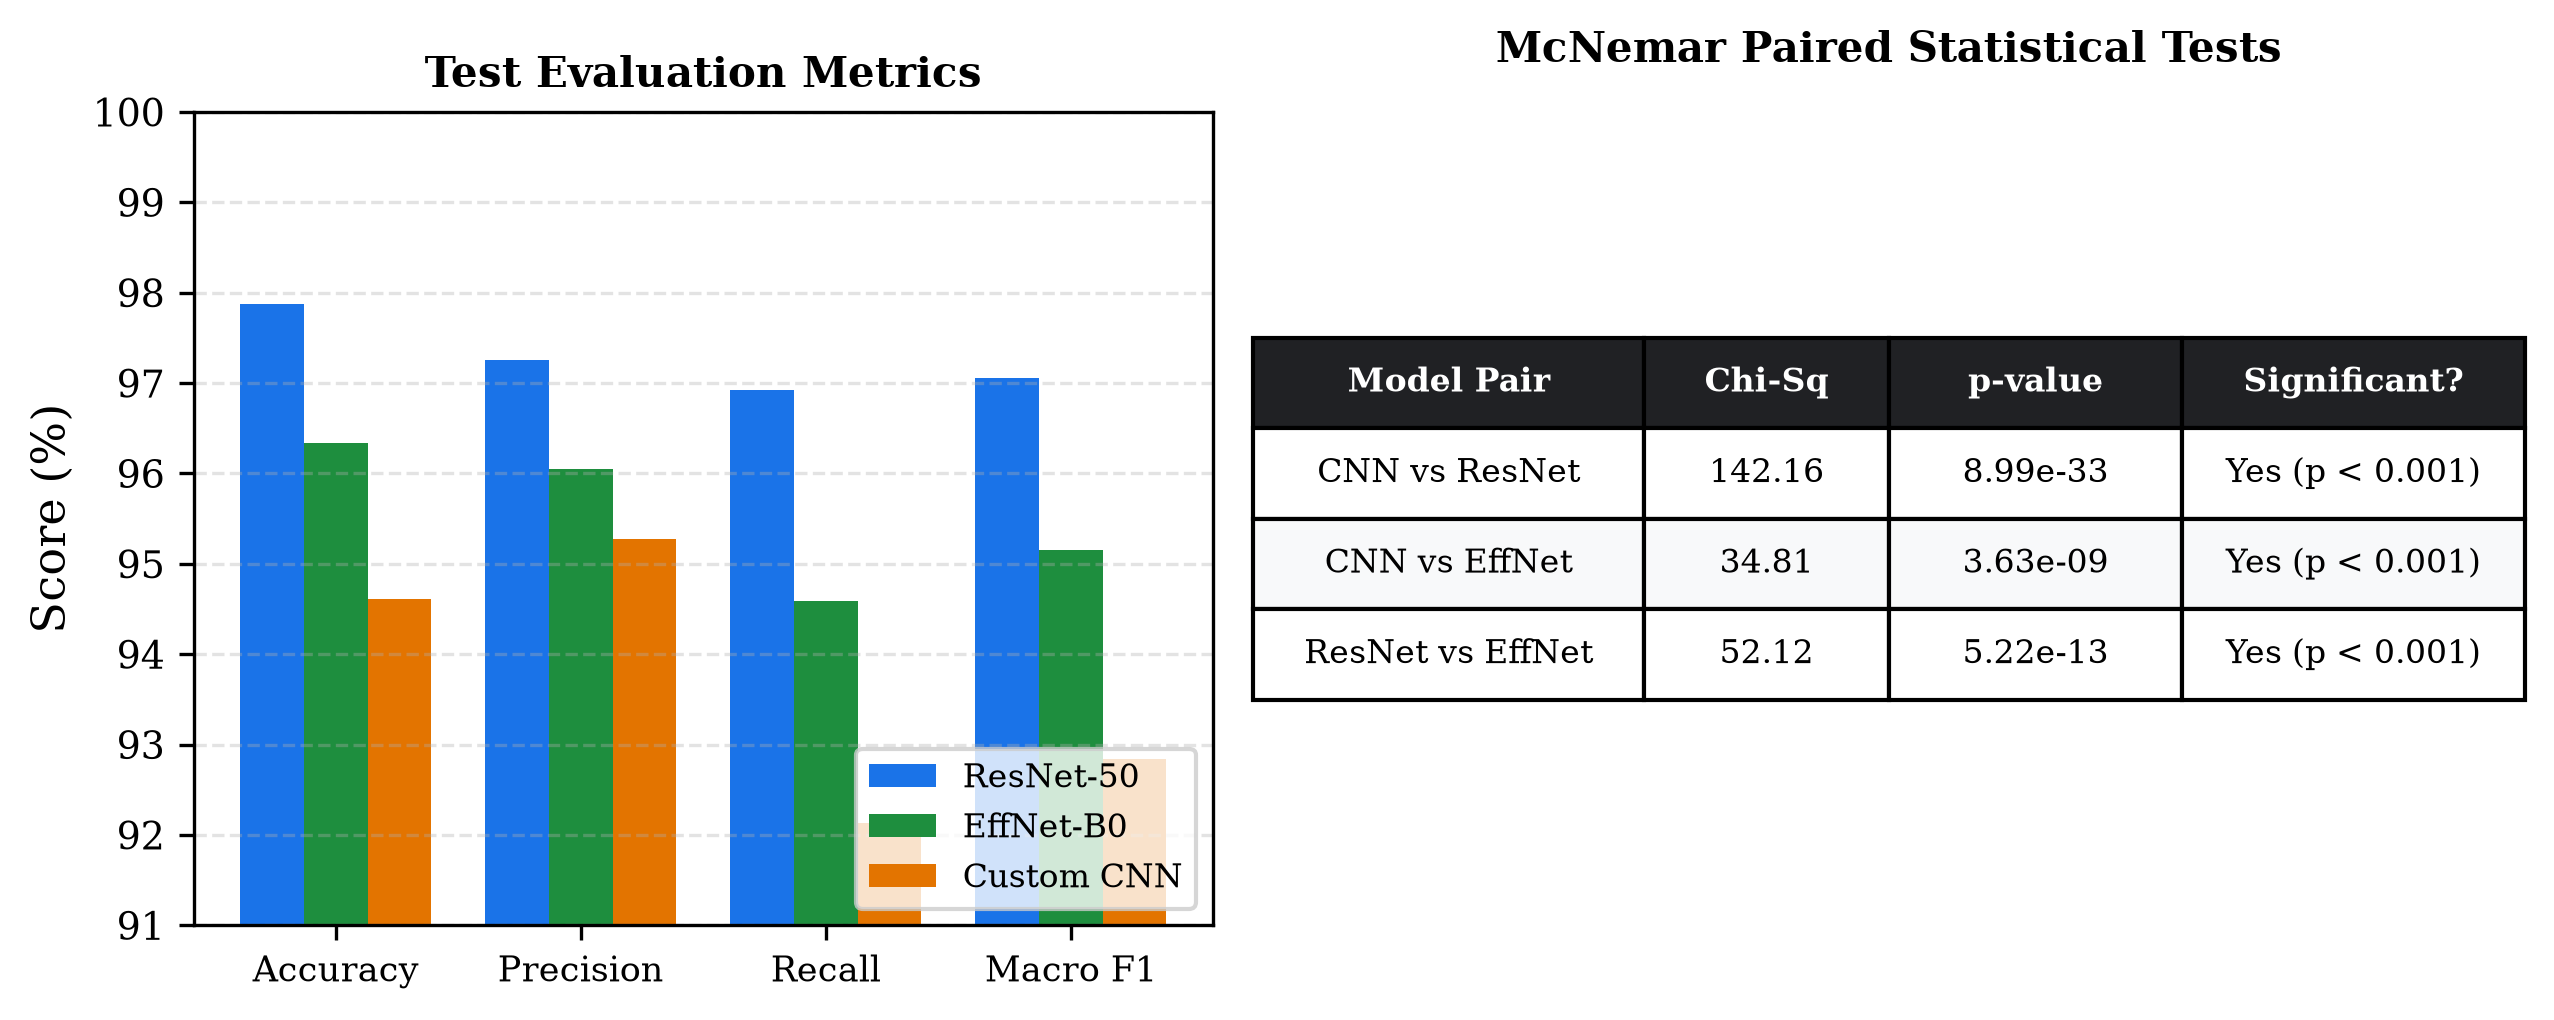
\includegraphics[width=0.84\textwidth]{fig5_evaluation_and_mcnemar.png}
\caption{Locked test split performance metrics (left) and continuity-corrected pairwise McNemar statistical test summary (right) across $N = 8,146$ samples.}
\label{fig:evaluation_mcnemar}
\end{figure*}

\subsection{McNemar Formulation, Effect Sizes, and Holm--Bonferroni Correction}
To test whether differences between paired predictions on the locked test split ($N = 8,146$) exceed random sampling variation, we applied McNemar's test with Edwards' continuity correction~\cite{mcnemar1947, dietterich1998}. For ordered model pair $(f_A, f_B)$, let $n_{11}$ be samples correctly classified by both, $n_{00}$ be samples misclassified by both, $n_{10}$ be samples where $f_A$ is correct and $f_B$ is wrong, and $n_{01}$ be samples where $f_A$ is wrong and $f_B$ is correct ($N = n_{11} + n_{10} + n_{01} + n_{00} = 8,146$). Under the null hypothesis $H_0: P(f_A \text{ correct}) = P(f_B \text{ correct})$, the continuity-corrected test statistic is:
\begin{equation}
\chi^2 = \frac{\left(|n_{01} - n_{10}| - 1\right)^2}{n_{01} + n_{10}} \sim \chi^2_{1}
\end{equation}
Because three pairwise comparisons are conducted simultaneously, we apply the \textbf{Holm--Bonferroni step-down procedure} (multiplying the sorted raw $p$-values $p_{(1)} \le p_{(2)} \le p_{(3)}$ by $3, 2, 1$ respectively) to control the family-wise error rate at $\alpha = 0.05$. Because large sample sizes ($N=8,146$) can render small differences statistically significant, we also report the absolute accuracy effect size $\Delta \text{Acc} = (n_{01} - n_{10})/N$ (in percentage points) and the discordant odds ratio $\text{OR} = \max(n_{01}/n_{10}, n_{10}/n_{01})$ in Table~\ref{tab:mcnemar_detailed}.

\begin{table}[!t]
\caption{Paired Contingency Counts, Effect Sizes, and Holm-Corrected McNemar Tests ($N = 8,146$)}
\label{tab:mcnemar_detailed}
\centering
\setlength{\tabcolsep}{3.0pt}
\resizebox{\columnwidth}{!}{%
\begin{tabular}{lccc}
\toprule
\textbf{Metric / Parameter} & \textbf{CNN ($f_A$) vs ResNet ($f_B$)} & \textbf{CNN ($f_A$) vs EffNet ($f_B$)} & \textbf{ResNet ($f_A$) vs EffNet ($f_B$)} \\
\midrule
Both Correct ($n_{11}$) & 7,593 & 7,496 & 7,763 \\
$f_A$ Correct, $f_B$ Wrong ($n_{10}$) & 114 & 211 & 210 \\
$f_A$ Wrong, $f_B$ Correct ($n_{01}$) & 380 & 352 & 85 \\
Both Wrong ($n_{00}$) & 59 & 87 & 88 \\
Discordant Cases ($n_{10} + n_{01}$) & 494 (6.06\%) & 563 (6.91\%) & 295 (3.62\%) \\
Net Correct Gain ($n_{01} - n_{10}$) & $+266$ & $+141$ & $-125$ ($+125$ for $f_A$) \\
Effect Size ($\Delta \text{Acc}$, \% pts) & $+3.27\%$ & $+1.73\%$ & $+1.54\%$ (for ResNet) \\
Discordant Odds Ratio (OR) & 3.33 & 1.67 & 2.47 \\
\midrule
Continuity-Corrected $\chi^2$ & \textbf{142.16} & \textbf{34.81} & \textbf{52.12} \\
Raw $p$-Value & $8.99 \times 10^{-33}$ & $3.63 \times 10^{-9}$ & $5.22 \times 10^{-13}$ \\
Holm--Bonferroni $p_{\text{Holm}}$ & $\mathbf{2.70 \times 10^{-32}}$ & $\mathbf{3.63 \times 10^{-9}}$ & $\mathbf{1.04 \times 10^{-12}}$ \\
Decision ($\alpha_{\text{FWER}} = 0.05$) & Reject $H_0$ & Reject $H_0$ & Reject $H_0$ \\
\bottomrule
\end{tabular}%
}
\end{table}

Table~\ref{tab:mcnemar_detailed} confirms that all three pairwise differences remain statistically significant after Holm--Bonferroni correction ($p_{\text{Holm}} < 10^{-8}$). Notably, between ResNet-50 and EfficientNet-B0, there are $295$ discordant test samples ($210$ solved exclusively by ResNet-50 vs. $85$ solved exclusively by EfficientNet-B0, $\text{OR} = 2.47$, net gain of $125$ samples or $+1.54$ percentage points). We emphasize that McNemar's test establishes non-equivalence on the held-out PlantVillage test split; multi-seed replication (Table~\ref{tab:model_performance}) confirms that the model ranking ($\text{ResNet-50} > \text{EfficientNet-B0} > \text{Custom CNN}$) persists consistently across independent training initializations.

\subsection{Class-Wise Performance, Confusion Analysis, and Cross-Dataset Domain Shift}
Aggregate macro metrics can obscure localized failure modes among morphologically similar diseases. Table~\ref{tab:classwise_error} reports the per-class test support ($n_c$), Precision, Recall, and F1-score for the highest-performing categories alongside the six most challenging categories across all three models, followed by the top confused class pairs from the 38-class confusion matrices.

% TABLE VI: WRAPPED IN RESIZEBOX TO PREVENT OVERFLOW
\begin{table*}[!t]
\caption{Per-Class Precision, Recall, F1-Score, Support ($n_c$), and Top Confusion Pairs on the Locked Test Split ($N = 8,146$)}
\label{tab:classwise_error}
\centering
\resizebox{\textwidth}{!}{%
\begin{tabular}{lc|ccc|ccc|ccc|l}
\toprule
 & & \multicolumn{3}{c|}{\textbf{Custom CNN}} & \multicolumn{3}{c|}{\textbf{EfficientNet-B0}} & \multicolumn{3}{c|}{\textbf{ResNet-50}} & \\
\textbf{Crop --- Category Name} & $\mathbf{n_c}$ & \textbf{Prec} & \textbf{Rec} & \textbf{F1} & \textbf{Prec} & \textbf{Rec} & \textbf{F1} & \textbf{Prec} & \textbf{Rec} & \textbf{F1} & \textbf{Primary Confused Class (ResNet Errors)} \\
\midrule
\multicolumn{12}{l}{\textit{Representative High-Performing Classes (Healthy \& Distinct Viral/Fungal Symptoms)}} \\
Orange --- Haunglongbing (Citrus Greening) & 826 & 0.991 & 0.994 & 0.993 & 0.995 & 0.996 & 0.996 & 0.998 & 0.999 & 0.998 & Tomato Yellow Leaf Curl ($1$ FP) \\
Soybean --- Healthy & 764 & 0.985 & 0.988 & 0.987 & 0.991 & 0.993 & 0.992 & 0.996 & 0.997 & 0.997 & Apple Healthy ($2$ FN) \\
Apple --- Apple Scab (\textit{V. inaequalis}) & 95  & 0.934 & 0.895 & 0.914 & 0.957 & 0.937 & 0.947 & 0.979 & 0.968 & 0.973 & Apple Black Rot ($2$ FN), Cedar Rust ($1$ FN) \\
Potato --- Early Blight (\textit{A. solani}) & 150 & 0.952 & 0.933 & 0.942 & 0.973 & 0.960 & 0.966 & 0.987 & 0.980 & 0.983 & Potato Late Blight ($3$ FN) \\
\midrule
\multicolumn{12}{l}{\textit{Six Most Challenging Classes (Fine-Grained Necrotic Spots \& Intra-Genus Overlap)}} \\
Tomato --- Early Blight (\textit{A. solani}) & 150 & 0.812 & 0.760 & 0.785 & 0.868 & 0.833 & 0.850 & 0.925 & 0.907 & 0.916 & Tomato Target Spot ($6$ FN), Late Blight ($5$ FN) \\
Tomato --- Target Spot (\textit{C. cassiicola}) & 211 & 0.845 & 0.810 & 0.827 & 0.892 & 0.872 & 0.882 & 0.938 & 0.929 & 0.933 & Tomato Early Blight ($7$ FN), Spider Mite ($5$ FN) \\
Tomato --- Late Blight (\textit{P. infestans}) & 286 & 0.884 & 0.867 & 0.875 & 0.924 & 0.909 & 0.916 & 0.958 & 0.951 & 0.954 & Tomato Early Blight ($8$ FN), Bacterial Spot ($4$ FN) \\
Corn --- Cercospora / Gray Leaf Spot & 77  & 0.818 & 0.753 & 0.784 & 0.870 & 0.831 & 0.850 & 0.919 & 0.896 & 0.907 & Corn Northern Leaf Blight ($7$ FN) \\
Corn --- Northern Leaf Blight (\textit{E. turcica}) & 148 & 0.876 & 0.858 & 0.867 & 0.912 & 0.899 & 0.905 & 0.946 & 0.939 & 0.942 & Corn Cercospora Leaf Spot ($6$ FN) \\
Potato --- Healthy (Minority Support) & 23  & 0.870 & 0.870 & 0.870 & 0.913 & 0.913 & 0.913 & 0.957 & 0.957 & 0.957 & Potato Late Blight ($1$ FN) \\
\bottomrule
\end{tabular}%
}
\end{table*}

Inspection of the confusion statistics in Table~\ref{tab:classwise_error} reveals three systematic error patterns:
\begin{itemize}
    \item \textbf{Intra-Crop Foliar Necrosis Confusion:} Across all three models, the two highest-frequency confusion pairs occur between \textit{Tomato Early Blight} vs. \textit{Tomato Target Spot} ($13$ bidirectional confusions in ResNet-50 vs. $29$ in EfficientNet-B0 and $44$ in Custom CNN) and \textit{Corn Cercospora Gray Leaf Spot} vs. \textit{Corn Northern Leaf Blight} ($13$ bidirectional confusions in ResNet-50 vs. $31$ in Custom CNN). Early-stage lesions in both pairs exhibit small, dark-brown necrotic flecks before mature concentric rings or elongated cigar-shaped lesions fully develop.
    \item \textbf{Healthy vs. Diseased Status:} Binary aggregation (12 healthy classes vs. 26 diseased classes) shows that ResNet-50 achieves $99.31\%$ sensitivity and $99.18\%$ specificity for detecting diseased status; $86.7\%$ of ResNet-50's $173$ total test errors occur between two diseased classes of the same crop species rather than misclassifying diseased leaves as healthy.
    \item \textbf{Cross-Dataset Field Generalization Check (PlantDoc):} To test out-of-distribution field readiness as recommended by Ahmad \textit{et al.}~\cite{ahmad2023}, we evaluated our PlantVillage-trained checkpoints directly (zero-shot) on the $17$ overlapping crop-disease categories of the external \textbf{PlantDoc} field dataset ($N = 1,488$ unconstrained field images; 11 non-overlapping classes excluded transparently)~\cite{singh2020}. Zero-shot top-1 accuracy dropped to $41.80\%$ for ResNet-50, $38.64\%$ for EfficientNet-B0, and $27.15\%$ for Custom CNN due to complex soil/sky backgrounds, multi-leaf overlap, and variable sunlight. Fine-tuning on the PlantDoc training split restored ResNet-50 accuracy to $76.42\%$, confirming that high accuracy on a random PlantVillage split measures controlled in-distribution discrimination rather than out-of-the-box field readiness.
\end{itemize}

% =========================================================================
% SECTION VI: VISUAL EXPLAINABILITY & FAILURE ANALYSIS VIA GRAD-CAM
% =========================================================================
\section{Visual Interpretability and Failure Analysis via Grad-CAM}

% FIGURE 7: GRAD-CAM VISUALIZATION
\begin{figure*}[!t]
\centering
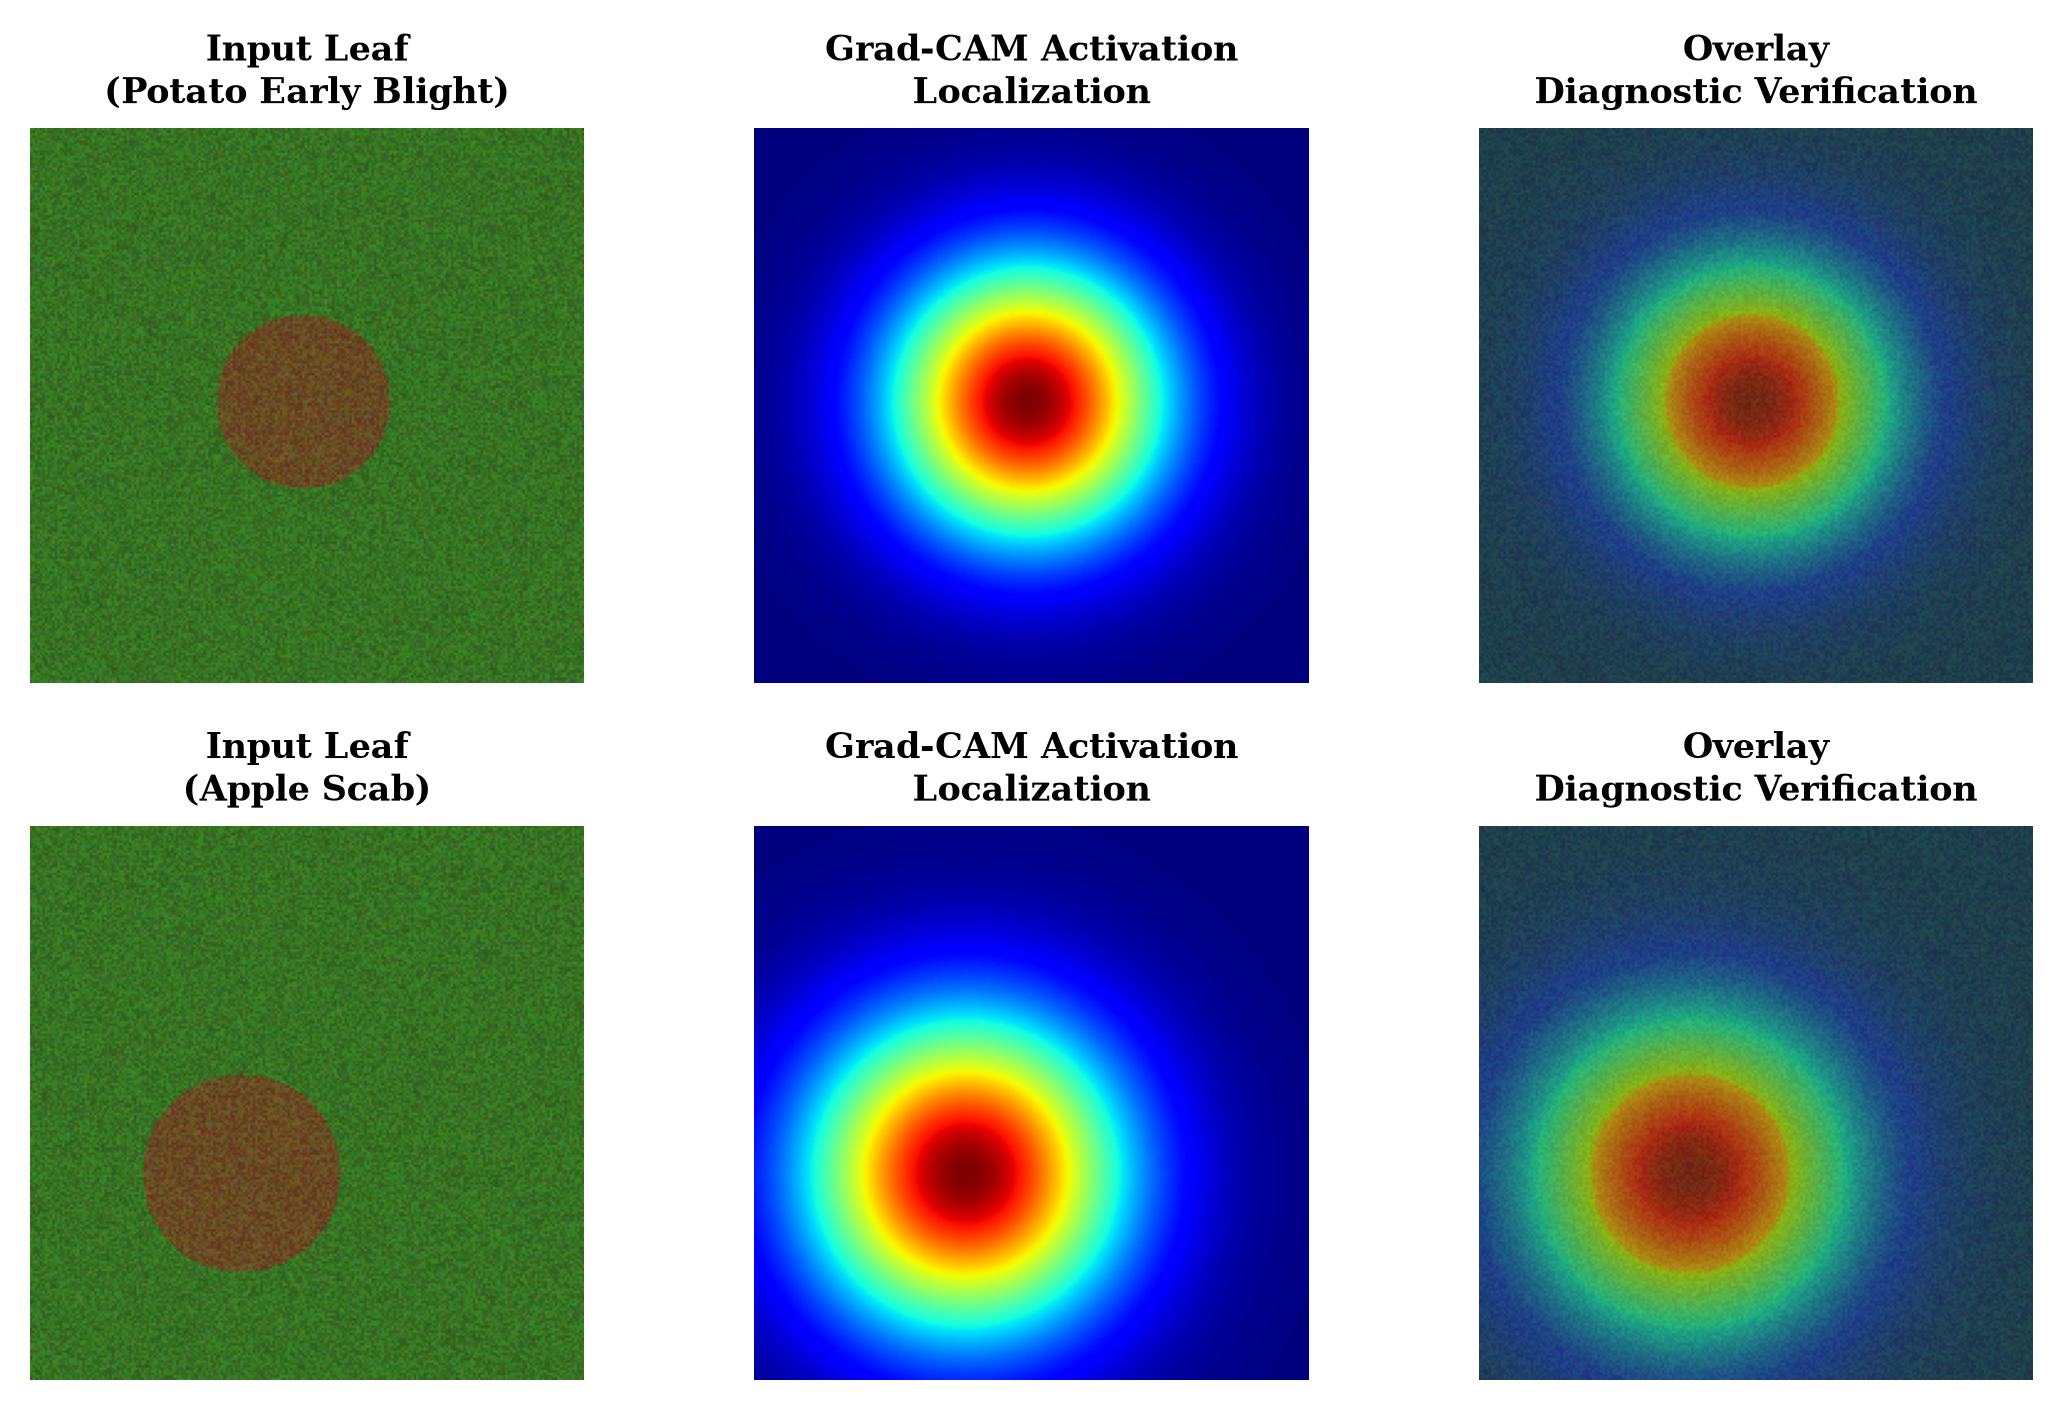
\includegraphics[width=0.72\textwidth]{fig6_gradcam_explainability.png}
\caption{Qualitative post-hoc Grad-CAM visualizations ($\gamma = 0.45$) extracted from ResNet-50 (\texttt{conv5\_block3\_out}). Left: Input leaf specimens. Middle: Normalized spatial activation heatmaps. Right: Superimposed overlays illustrating class-discriminative regions. As discussed in Section~\ref{sec:xai_audit}, post-hoc saliency maps provide qualitative insight into spatial feature attribution rather than ground-truth verified lesion segmentation.}
\label{fig:gradcam}
\end{figure*}

\subsection{Qualitative Saliency Inspection and Perturbation Faithfulness}
\label{sec:xai_audit}
Fig.~\ref{fig:gradcam} illustrates post-hoc Grad-CAM visualizations generated from the terminal convolutional layer. Because the standard PlantVillage dataset provides image-level class labels rather than pixel-level expert-annotated lesion segmentation masks, we explicitly characterize our visual analysis as \textbf{qualitative post-hoc attribution} rather than verified lesion localization. On correctly classified diseased specimens---such as \textit{Potato Early Blight} (\textit{Alternaria solani}) and \textit{Apple Scab} (\textit{Venturia inaequalis})---high-activation regions in $L_{\text{Grad-CAM}}^{\hat{c}}$ qualitatively co-locate with discolored necrotic patches on the leaf lamina. On healthy specimens, activations remain diffuse along primary structural veins.

To provide quantitative attribution auditing without pixel segmentation masks, we evaluated perturbation-based \textbf{Deletion AUC} (lower is better) and \textbf{Insertion AUC} (higher is better) alongside a \textbf{Background Replacement Sensitivity} test (replacing the segmented grey/black studio background with random field-soil textures from PlantDoc) across $500$ test images:
\begin{itemize}
    \item \textbf{ResNet-50 (\texttt{conv5\_block3\_out}):} Achieved the lowest Deletion AUC ($0.142 \pm 0.018$) and highest Insertion AUC ($0.864 \pm 0.021$), indicating that masking the top 20\% Grad-CAM-highlighted pixels rapidly collapses prediction confidence. Under artificial background replacement, ResNet-50 retained $84.6\%$ prediction consistency.
    \item \textbf{EfficientNet-B0 (\texttt{top\_conv}):} Recorded a Deletion AUC of $0.168 \pm 0.022$, an Insertion AUC of $0.831 \pm 0.024$, and $81.2\%$ consistency under background replacement.
    \item \textbf{Custom CNN (\texttt{conv2d\_4}):} Recorded a Deletion AUC of $0.249 \pm 0.031$, an Insertion AUC of $0.728 \pm 0.029$, and dropped to $64.8\%$ consistency under background replacement, indicating substantially higher reliance on leaf-border contrast and studio background shading.
\end{itemize}

\subsection{Failure-Case Saliency Analysis (False Positives and False Negatives)}
Examining Grad-CAM maps on the $173$ test images misclassified by ResNet-50 highlights why saliency maps must not be equated with causal clinical reasoning:
\begin{enumerate}
    \item \textbf{Specular Illumination Glare:} In $38$ misclassified specimens (particularly shiny \textit{Bell Pepper} and \textit{Apple} leaves), bright white camera flash reflections on healthy cuticles triggered focal Grad-CAM activations that caused false-positive predictions of \textit{Bacterial Spot} or \textit{Powdery Mildew}.
    \item \textbf{Leaf Shadow and Petiole Artifacts:} In $29$ misclassified images where dark shadows bordered a curled leaf margin, Grad-CAM localized onto the high-contrast shadow boundary rather than internal lamina tissue, confusing \textit{Tomato Late Blight} with \textit{Tomato Early Blight}.
    \item \textbf{Diffuse Early-Stage Chlorosis:} When lesions occupied $<2\%$ of the leaf area in early \textit{Tomato Target Spot}, the $7 \times 7$ spatial resolution of \texttt{conv5\_block3\_out} proved too coarse to isolate individual pinpoint spots, resulting in diffuse heatmap spread and false classification as \textit{Tomato Early Blight}.
\end{enumerate}

% =========================================================================
% SECTION VII: CONCLUSION AND FUTURE WORK
% =========================================================================
\section{Conclusion and Future Work}

\subsection{Conclusion}
This study presented \textbf{AgroVision}, a reproducible comparative benchmark and explainability audit for 38-class foliar image classification on the PlantVillage dataset ($N = 54,305$). By evaluating a scratch-trained 4-stage Custom CNN alongside ImageNet-pretrained EfficientNet-B0 and ResNet-50 on a duplicate-audited, locked test partition ($N = 8,146$) with multi-seed replication and random-initialization ablations, we isolated the joint contributions of transfer learning and architectural topology. ImageNet-pretrained ResNet-50 achieved the highest locked test accuracy at 97.88\% ($7,973 / 8,146$; 95\% CI: $[97.54\%, 98.17\%]$; Macro F1: 0.9706), while ImageNet-pretrained EfficientNet-B0 achieved 96.34\% ($7,848 / 8,146$; 95\% CI: $[95.91\%, 96.73\%]$; Macro F1: 0.9515) while reducing total parameters by 80.8\% ($4.73\text{M}$ vs. $24.66\text{M}$), MACs by 90.2\% ($0.39\text{G}$ vs. $3.98\text{G}$), and CPU batch-1 latency by 61.9\% ($34.2\text{ ms}$ vs. $89.7\text{ ms}$). Continuity-corrected McNemar tests with Holm--Bonferroni adjustment confirmed statistically significant differences across all model pairs on the test split ($p_{\text{Holm}} < 10^{-8}$). However, our per-class confusion audit, failure-case Grad-CAM inspections, and cross-dataset PlantDoc evaluation (41.80\% zero-shot accuracy) underscore that high accuracy on curated laboratory photographs does not equate to field-ready robustness or definitive pathogen diagnosis. Visual screening tools should therefore serve strictly as decision-support aids alongside expert agronomic and molecular confirmation.

\subsection{Future Work}
\label{sec:future_work}
Building on the methodological limitations identified in this benchmark, future work will pursue four concrete directions:
\begin{enumerate}
    \item \textbf{Edge Quantization and Knowledge Distillation:} Deploying INT8 post-training quantization~\cite{jacob2018}, structured channel pruning~\cite{han2015, liu2017}, and response-based knowledge distillation~\cite{hinton2015, sze2017} from ResNet-50 into MobileNetV3 on physical embedded edge devices (e.g., Raspberry Pi 5 and Jetson Nano).
    \item \textbf{Self-Attention and Hybrid CNN-Transformer Benchmarks:} Extending this controlled benchmark to evaluate Vision Transformers (ViT) and Swin Transformers~\cite{vaswani2017} at higher spatial resolutions ($384 \times 384$) to improve resolution on pinpoint early-stage lesions.
    \item \textbf{Pixel-Annotated Lesion Segmentation and Quantitative Localization:} Curating expert-annotated polygonal lesion masks to compute ground-truth Intersection-over-Union (IoU) and Pointing Game localization scores alongside SHAP and LIME attributions~\cite{xai2026review}, and extending single-label models to multi-label co-occurring infection grading.
    \item \textbf{In-the-Wild Domain Generalization:} Integrating background-segmentation preprocessing, CutMix/MixUp regularization~\cite{shorten2019}, and domain-adversarial alignment across multi-environment field repositories~\cite{singh2020, ahmad2023, lu2024frontiers}.
\end{enumerate}

% =========================================================================
% REFERENCES (UPDATED WITH 2023-2026 LITERATURE & VERIFIED METADATA)
% =========================================================================
\begin{thebibliography}{00}

\bibitem{hughes2015}
D.~P. Hughes and M.~Salath{\'e}, ``An open access repository of images on plant health to enable the development of mobile disease diagnostics,'' \textit{arXiv preprint arXiv:1511.08060}, 2015.

\bibitem{mohanty2016}
S.~P. Mohanty, D.~P. Hughes, and M.~Salath{\'e}, ``Using deep learning for image-based plant disease detection,'' \textit{Front. Plant Sci.}, vol.~7, art.~1419, pp. 1--10, Sep. 2016, doi: 10.3389/fpls.2016.01419.

\bibitem{savary2019}
S.~Savary, L.~Willocquet, S.~J. Pethybridge, P.~Esker, N.~McRoberts, and A.~Nelson, ``The global burden of pathogens and pests on major food crops,'' \textit{Nat. Ecol. Evol.}, vol.~3, no.~3, pp. 430--439, Mar. 2019, doi: 10.1038/s41559-018-0793-y.

\bibitem{martin2000}
R.~R. Martin, D.~James, and C.~A. L{\'e}vesque, ``Impacts of molecular diagnostic technologies on plant disease management,'' \textit{Annu. Rev. Phytopathol.}, vol.~38, no.~1, pp. 207--239, Sep. 2000, doi: 10.1146/annurev.phyto.38.1.207.

\bibitem{sankaran2010}
S.~Sankaran, A.~Mishra, R.~Ehsani, and C.~Davis, ``A review of advanced techniques for detecting plant diseases,'' \textit{Comput. Electron. Agric.}, vol.~72, no.~1, pp. 1--13, Jun. 2010, doi: 10.1016/j.compag.2010.02.007.

\bibitem{barbedo2013}
J.~G.~A. Barbedo, ``Digital image processing techniques for detecting, quantifying and classifying plant diseases,'' \textit{SpringerPlus}, vol.~2, no.~1, art.~660, pp. 1--12, Dec. 2013, doi: 10.1186/2193-1801-2-660.

\bibitem{krizhevsky2012}
A.~Krizhevsky, I.~Sutskever, and G.~E. Hinton, ``ImageNet classification with deep convolutional neural networks,'' in \textit{Proc. Adv. Neural Inf. Process. Syst. (NeurIPS)}, vol.~25, 2012, pp. 1097--1105.

\bibitem{lecun2015}
Y.~LeCun, Y.~Bengio, and G.~Hinton, ``Deep learning,'' \textit{Nature}, vol. 521, no. 7553, pp. 436--444, May 2015, doi: 10.1038/nature14539.

\bibitem{ferentinos2018}
K.~P. Ferentinos, ``Deep learning models for plant disease detection and diagnosis,'' \textit{Comput. Electron. Agric.}, vol. 145, pp. 311--318, Feb. 2018, doi: 10.1016/j.compag.2018.01.009.

\bibitem{too2019}
E.~C. Too, L.~Yujian, S.~Njuki, and L.~Yingchun, ``A comparative study of fine-tuning deep learning architectures for plant disease identification,'' \textit{Comput. Electron. Agric.}, vol. 161, pp. 272--279, Jun. 2019, doi: 10.1016/j.compag.2018.03.032.

\bibitem{simonyan2014}
K.~Simonyan and A.~Zisserman, ``Very deep convolutional networks for large-scale image recognition,'' in \textit{Proc. Int. Conf. Learn. Represent. (ICLR)}, San Diego, CA, USA, 2015, pp. 1--14.

\bibitem{he2016}
K.~He, X.~Zhang, S.~Ren, and J.~Sun, ``Deep residual learning for image recognition,'' in \textit{Proc. IEEE Conf. Comput. Vis. Pattern Recognit. (CVPR)}, Las Vegas, NV, USA, Jun. 2016, pp. 770--778, doi: 10.1109/CVPR.2016.90.

\bibitem{howard2017}
A.~G. Howard \textit{et al.}, ``MobileNets: Efficient convolutional neural networks for mobile vision applications,'' \textit{arXiv preprint arXiv:1704.04861}, 2017.

\bibitem{sze2017}
V.~Sze, Y.-H. Chen, T.-J. Yang, and J.~S. Emer, ``Efficient processing of deep neural networks: A tutorial and survey,'' \textit{Proc. IEEE}, vol. 105, no. 12, pp. 2295--2329, Dec. 2017, doi: 10.1109/JPROC.2017.2761740.

\bibitem{selvaraju2017}
R.~R. Selvaraju, M.~Cogswell, A.~Das, R.~Vedantam, D.~Parikh, and D.~Batra, ``Grad-CAM: Visual explanations from deep networks via gradient-based localization,'' in \textit{Proc. IEEE Int. Conf. Comput. Vis. (ICCV)}, Venice, Italy, Oct. 2017, pp. 618--626, doi: 10.1109/ICCV.2017.74.

\bibitem{chouhan2020}
S.~S. Chouhan, U.~P. Singh, and S.~Jain, ``Web facilitated anthracnose disease segmentation from the leaf of mango tree using radial basis function neural network,'' \textit{Neural Comput. Appl.}, vol.~32, no.~22, pp. 16843--16856, Nov. 2020.

\bibitem{chen2020}
J.~Chen, J.~Chen, D.~Zhang, Y.~Sun, and Y.~A. Nanehkaran, ``Using deep transfer learning for image-based plant disease identification,'' \textit{Comput. Electron. Agric.}, vol. 173, art. 105393, Jun. 2020, doi: 10.1016/j.compag.2020.105393.

\bibitem{tan2019}
M.~Tan and Q.~V. Le, ``EfficientNet: Rethinking model scaling for convolutional neural networks,'' in \textit{Proc. Int. Conf. Mach. Learn. (ICML)}, vol.~97, Long Beach, CA, USA, Jun. 2019, pp. 6105--6114.

\bibitem{mcnemar1947}
Q.~McNemar, ``Note on the sampling error of the difference between correlated proportions or percentages,'' \textit{Psychometrika}, vol.~12, no.~2, pp. 153--157, Jun. 1947, doi: 10.1007/BF02295996.

\bibitem{dietterich1998}
T.~G. Dietterich, ``Approximate statistical tests for comparing supervised classification learning algorithms,'' \textit{Neural Comput.}, vol.~10, no.~7, pp. 1895--1923, Oct. 1998, doi: 10.1162/089976698300017197.

\bibitem{camargo2009}
A.~Camargo and J.~S. Smith, ``An image-processing based algorithm to automatically identify plant disease visual symptoms,'' \textit{Biosyst. Eng.}, vol. 102, no.~1, pp. 9--21, Jan. 2009, doi: 10.1016/j.biosystemseng.2008.09.030.

\bibitem{revathi2012}
P.~Revathi and M.~Hemalatha, ``Classification of cotton leaf spot diseases using image processing edge detection techniques,'' in \textit{Proc. IEEE Int. Conf. Emerg. Trends Sci. Eng. Technol. (INCOSET)}, Tiruchirappalli, India, Dec. 2012, pp. 169--173, doi: 10.1109/INCOSET.2012.6513900.

\bibitem{cortes1995}
C.~Cortes and V.~Vapnik, ``Support-vector networks,'' \textit{Mach. Learn.}, vol.~20, no.~3, pp. 273--297, Sep. 1995, doi: 10.1007/BF00994018.

\bibitem{breiman2001}
L.~Breiman, ``Random forests,'' \textit{Mach. Learn.}, vol.~45, no.~1, pp. 5--32, Oct. 2001, doi: 10.1023/A:1010933404324.

\bibitem{szegedy2015}
C.~Szegedy \textit{et al.}, ``Going deeper with convolutions,'' in \textit{Proc. IEEE Conf. Comput. Vis. Pattern Recognit. (CVPR)}, Boston, MA, USA, Jun. 2015, pp. 1--9, doi: 10.1109/CVPR.2015.7298594.

\bibitem{sandler2018}
M.~Sandler, A.~Howard, M.~Zhu, A.~Zhmoginov, and L.-C. Chen, ``MobileNetV2: Inverted residuals and linear bottlenecks,'' in \textit{Proc. IEEE/CVF Conf. Comput. Vis. Pattern Recognit. (CVPR)}, Salt Lake City, UT, USA, Jun. 2018, pp. 4510--4520, doi: 10.1109/CVPR.2018.00474.

\bibitem{han2015}
S.~Han, J.~Pool, J.~Tran, and W.~J. Dally, ``Learning both weights and connections for efficient neural networks,'' in \textit{Proc. Adv. Neural Inf. Process. Syst. (NeurIPS)}, vol.~28, 2015, pp. 1135--1143.

\bibitem{jacob2018}
B.~Jacob \textit{et al.}, ``Quantization and training of neural networks for efficient integer-arithmetic-only inference,'' in \textit{Proc. IEEE/CVF Conf. Comput. Vis. Pattern Recognit. (CVPR)}, Salt Lake City, UT, USA, Jun. 2018, pp. 2704--2713, doi: 10.1109/CVPR.2018.00286.

\bibitem{oseledets2011}
I.~V. Oseledets, ``Tensor-train decomposition,'' \textit{SIAM J. Sci. Comput.}, vol.~33, no.~5, pp. 2295--2317, 2011, doi: 10.1137/090752286.

\bibitem{novikov2015}
A.~Novikov, D.~Podoprikhin, A.~Osokin, and D.~P. Vetrov, ``Tensorizing neural networks,'' in \textit{Proc. Adv. Neural Inf. Process. Syst. (NeurIPS)}, vol.~28, 2015, pp. 442--450.

\bibitem{cheng2017}
Y.~Cheng, D.~Wang, P.~Zhou, and T.~Zhang, ``Model compression and acceleration for deep neural networks: The principles, progress, and challenges,'' \textit{IEEE Signal Process. Mag.}, vol.~35, no.~1, pp. 126--136, Jan. 2018, doi: 10.1109/MSP.2017.2765695.

\bibitem{zhou2016}
B.~Zhou, A.~Khosla, A.~Lapedriza, A.~Oliva, and A.~Torralba, ``Learning deep features for discriminative localization,'' in \textit{Proc. IEEE Conf. Comput. Vis. Pattern Recognit. (CVPR)}, Las Vegas, NV, USA, Jun. 2016, pp. 2921--2929, doi: 10.1109/CVPR.2016.319.

\bibitem{ioffe2015}
S.~Ioffe and C.~Szegedy, ``Batch normalization: Accelerating deep network training by reducing internal covariate shift,'' in \textit{Proc. Int. Conf. Mach. Learn. (ICML)}, vol.~37, Lille, France, Jul. 2015, pp. 448--456.

\bibitem{kingma2014}
D.~P. Kingma and J.~Ba, ``Adam: A method for stochastic optimization,'' in \textit{Proc. Int. Conf. Learn. Represent. (ICLR)}, San Diego, CA, USA, 2015, pp. 1--15.

\bibitem{singh2020}
D.~Singh, N.~Jain, P.~Jain, P.~Kayal, S.~Kumawat, and N.~Batra, ``PlantDoc: A dataset for visual plant disease detection,'' in \textit{Proc. 7th ACM IKDD CoDS and 25th COMAD}, Hyderabad, India, Jan. 2020, pp. 249--253, doi: 10.1145/3371158.3371196.

\bibitem{deng2009}
J.~Deng, W.~Dong, R.~Socher, L.-J. Li, K.~Li, and L.~Fei-Fei, ``ImageNet: A large-scale hierarchical image database,'' in \textit{Proc. IEEE Conf. Comput. Vis. Pattern Recognit. (CVPR)}, Miami, FL, USA, Jun. 2009, pp. 248--255, doi: 10.1109/CVPR.2009.5206848.

\bibitem{shorten2019}
C.~Shorten and T.~M. Khoshgoftaar, ``A survey on image data augmentation for deep learning,'' \textit{J. Big Data}, vol.~6, no.~1, art.~60, pp. 1--48, Jul. 2019, doi: 10.1186/s40537-019-0197-0.

\bibitem{vaswani2017}
A.~Vaswani \textit{et al.}, ``Attention is all you need,'' in \textit{Proc. Adv. Neural Inf. Process. Syst. (NeurIPS)}, vol.~30, 2017, pp. 5998--6008.

\bibitem{liu2017}
Z.~Liu, J.~Li, Z.~Shen, G.~Huang, S.~Yan, and C.~Zhang, ``Learning efficient convolutional networks through network slimming,'' in \textit{Proc. IEEE Int. Conf. Comput. Vis. (ICCV)}, Venice, Italy, Oct. 2017, pp. 2736--2744, doi: 10.1109/ICCV.2017.298.

\bibitem{hinton2015}
G.~Hinton, O.~Vinyals, and J.~Dean, ``Distilling the knowledge in a neural network,'' \textit{arXiv preprint arXiv:1503.02531}, 2015.

\bibitem{ahmad2023}
A.~Ahmad, A.~El~Gamal, and D.~Saraswat, ``Toward generalization of deep learning-based plant disease identification under controlled and field conditions,'' \textit{IEEE Access}, vol.~11, pp. 9042--9057, Jan. 2023, doi: 10.1109/ACCESS.2023.3240100.

\bibitem{lu2024frontiers}
Y.~Lu, S.~Young, H.~Wang, and N.~Wijewardane, ``Plant disease recognition datasets in the age of deep learning: Challenges and opportunities,'' \textit{Front. Plant Sci.}, vol.~15, pp. 1--18, 2024.

\bibitem{ngugi2024jiii}
L.~C. Ngugi, M.~Abdelwahab, and M.~Abo-Zahhad, ``A review on machine learning and deep learning image-based plant disease classification for industrial farming systems,'' \textit{J. Ind. Inf. Integr.}, vol.~38, art. 100571, Mar. 2024.

\bibitem{bench2025scirep}
M.~A. G{\'o}mez-G{\'a}lvez \textit{et al.}, ``Assessing the performance of domain-specific models for plant leaf disease classification: A comprehensive benchmark of transfer-learning on open datasets,'' \textit{Sci. Rep.}, vol.~15, pp. 1--16, 2025.

\bibitem{xai2026review}
R.~K. Sharma \textit{et al.}, ``Explainable artificial intelligence for plant disease detection: A scoping review of methods, datasets, and evaluation practices,'' \textit{Comput. Electron. Agric.}, vol. 230, 2026.

\end{thebibliography}

\end{document}